\documentclass[11pt,a4paper,twoside,openright]{report}

\usepackage[italian]{babel}
\usepackage[utf8]{inputenc}
\usepackage{graphicx}
\usepackage{tabularx}
\usepackage{subfigure}
\usepackage{afterpage}
\usepackage{amsmath,amssymb}            
\usepackage{rotating}  
\usepackage{fancyhdr}  
\usepackage[scriptsize]{caption}
\usepackage{csquotes}
\usepackage{listings}
\usepackage{color}
\usepackage[backend=bibtex,style=numeric-comp]{biblatex}

\addbibresource{bibl_tesi.bib}

\setlength{\paperwidth}{16cm}
\setlength{\paperheight}{22cm}
\setlength{\oddsidemargin} {2. cm}
\setlength{\evensidemargin} {2. cm}
\addtolength{\oddsidemargin} {-0.4 cm}
\addtolength{\evensidemargin} {-0.4 cm}

\renewcommand{\captionfont}{\normalfont \sffamily \itshape \small}

\lstloadlanguages{C,Java,[CORBA]IDL,[GNU]C++,SQL}

\definecolor{codegreen}{rgb}{0,0.6,0}
\definecolor{codegray}{rgb}{0.5,0.5,0.5}
\definecolor{codepurple}{rgb}{0.58,0,0.82}

\lstset{basicstyle=\small\ttfamily,
	keywordstyle=\color{blue}\bfseries,
	commentstyle=\color{green},
	stringstyle=\color{red},
	showstringspaces=true,
	numbers=left,
	frame=single,
	columns=fullflexible,
	breaklines=true,
	float=tb,
	captionpos=b}

\newcommand{\lstname}{Listato }

\pagestyle{empty}

\begin{document}
\thispagestyle{empty}
%\begin{titlepage}
\vspace*{-1.5cm} \bfseries{
\begin{center}
  \large
  POLITECNICO DI MILANO\\
  \normalsize
  Corso di Laurea \textbf{(MAGISTRALE ?)} in Ingegneria Informatica\\
  Dipartimento di Elettronica e Informazione\\
  \begin{figure}[htbp]
    \begin{center}
      
\includegraphics[width=3.5cm]{./pictures/logopm}
%	
\psfig{file=./pictures/logopm.jpg,width=3.5cm}
    \end{center}
  \end{figure}
  \vspace*{0.3cm} \LARGE



  \textbf{TITOLO DELLA TESI}\\



  \vspace*{.75truecm} \large
  AI \& R Lab \\
  Laboratorio di Intelligenza Artificiale \\
  e Robotica del Politecnico di Milano
\end{center}
\vspace*{3.0cm} \large
\begin{flushleft}


  Relatore: Ing. Matteo Matteucci \\
  Correlatore: Prof. Andrea Bonarini 

\end{flushleft}
\vspace*{1.0cm}
\begin{flushright}


  Tesi di Laurea di:\\ Bud Spencer, matricola 634845 \\ 
		       Terence Hill, matricola 641067 \\


\end{flushright}
\vspace*{0.5cm}
\begin{center}



  Anno Accademico 200N-200N+1
\end{center} \clearpage
}

\thispagestyle{empty} \normalfont \cleardoublepage
\vspace{17cm}

%\large
\begin{flushright}
\itshape{ A Ilaria}
\end{flushright}

\thispagestyle{empty}  \cleardoublepage
\pagenumbering{Roman}
\newpage
\chapter*{Sommario}

\addcontentsline{toc}{chapter}{Sommario}

Questa tesi è stata sviluppata in collaborazione con \emph{LIS S.p.a.}, vigilanza privata che si distingue per i tempi di intervento ridotti e la possibilità di gestione degli impianti da remoto. Queste caratteristiche distinguono LIS già dai primi anni di attività quando ancora la ricezione degli allarmi e la telegestione avveniva tramite linee telefoniche tradizionali.
Negli ultimi anni, tuttavia, la scomparsa delle linee telefoniche tradizionali in favore di quelle VoIP e di connessioni in fibra ottica hanno creato diversi problemi alla normale ricezione degli allarmi e ai meccanismi di telegestione.
Lo scopo di questa tesi è quello di progettare e realizzare un sistema di ricezione allarmi e telegestione unificato che sia tuttavia modulare, che utilizzi nuovi canali di comunicazione e che possa essere integrato con il software preesistente.
Nel seguito vedremo come questo lavoro ci ha permesso di ridurre i tempi di integrazione di nuovi metodi di ricezione e telegestione e di aumentare conseguentemente il numero di centrali connesse e gestite dalla centrale operativa.

\thispagestyle{empty} \vspace*{.75truecm} \cleardoublepage
\chapter*{Ringraziamenti}

\addcontentsline{toc}{chapter}{Ringraziamenti}

Ringrazio innanzitutto il Prof. William Fornaciari senza il quale questa tesi non sarebbe nemmeno iniziata e che grazie alla sua grande esperienza mi ha aiutato a concluderla.\\
Ringrazio poi LIS S.p.a. nelle figure di Andrea Ziliani, Damiano Roda, Emanuele Gagliano che mi hanno dato gli strumenti e la libertà di realizzare questa tesi in piena autonomia. Ringrazio Massimiliono Zanzottera, gli operatori di centrale e i collaudatori che mi hanno aiutato ad addentrarmi nel mondo della vigilanza privata. Ringrazio infine Alessandro Gelormini, collega che insieme a me ha sviluppato il software presente in LIS soprattutto tutto il comparto Java.\\
Ringrazio la mia famiglia che mi ha spronato a portare a trmmine questo compito, e ringrazio Ilaria che mi ha sempre supportato.
Infine ringrazio tutti i miei amici e compagni di corso che hanno reso questa esperienza se non meno dura almeno più allegra.

\thispagestyle{empty} \vspace*{.75truecm} \normalfont \cleardoublepage
\pagenumbering{arabic}

\tableofcontents

\pagestyle{fancy} 
\fancyfoot{}
\renewcommand{\chaptermark}[1]{\markboth{\chaptername\ \thechapter.\ #1}{}} 
\renewcommand{\sectionmark}[1]{\markright{\thesection.\ #1}}         
\fancyhead[LE,RO]{\bfseries\thepage}    
                                        
\fancyhead[RE]{\bfseries\leftmark}    
\fancyhead[LO]{\bfseries\rightmark}     
\renewcommand{\headrulewidth}{0.3pt} 

\chapter{Introduzione}
\label{Introduzione}
\thispagestyle{empty}

\begin{quotation}
{\footnotesize
\noindent{\emph{``Terence: Rotta a nord con circospezione \\
Bud: Ehi, gli ordini li do io qui!\\
Terence: Ok, comante\\
Bud: Rotta a nord\\
Terence: Soltanto?\\
Bud: Con circospezione!''}
}
\begin{flushright}
Chi Trova un Amico Trova un Tesoro
\end{flushright}
}
\end{quotation}
\vspace{0.5cm}

\noindent L'introduzione deve essere atomica, quindi non deve contenere n\`e sottosezioni n\`e paragrafi n\`e altro. Il titolo, il sommario e l'introduzione devono sembrare delle scatole cinesi, nel senso che lette in quest'ordine devono progressivamente svelare informazioni sul contenuto per incatenare l'attenzione del lettore e indurlo a leggere l'opera fino in fondo. L'introduzione deve essere tripartita, non graficamente ma logicamente:

\section{Inquadramento generale}
La prima parte contiene una frase che spiega l'area generale dove si svolge il lavoro; una che spiega la sottoarea pi\`u specifica dove si svolge il lavoro e la terza, che dovrebbe cominciare con le seguenti parole ``lo scopo della tesi \`e \dots'', illustra l'obbiettivo del lavoro. Poi vi devono essere una o due frasi che contengano una breve spiegazione di cosa e come \`e stato fatto, delle attivit\`a� sperimentali, dei risultati ottenuti con una valutazione e degli sviluppi futuri. La prima parte deve essere circa una facciata e mezza o due

\section{Breve descrizione del lavoro}
La seconda parte deve essere una esplosione della prima e deve quindi mostrare in maniera pi\`u esplicita l'area dove si svolge il lavoro, le fonti bibliografiche pi\`u importanti su cui si fonda il lavoro in maniera sintetica (una pagina) evidenziando i lavori in letteratura che presentano attinenza con il lavoro affrontato in modo da mostrare da dove e perch\'e \`e sorta la tematica di studio. Poi si mostrano esplicitamente le realizzazioni, le direttive future di ricerca, quali sono i problemi aperti e quali quelli affrontati e si ripete lo scopo della tesi. Questa parte deve essere piena (ma non grondante come la sezione due) di citazioni bibliografiche e deve essere lunga circa 4 facciate.

\section{Struttura della tesi}
La terza parte contiene la descrizione della struttura della tesi ed \`e organizzata nel modo seguente.
``La tesi \`e strutturata nel modo seguente.

Nella sezione due si mostra \dots

Nella sez. tre si illustra \dots

Nella sez. quattro si descrive \dots

Nelle conclusioni si riassumono gli scopi, le valutazioni di questi e le prospettive future \dots

Nell'appendice A si riporta \dots (Dopo ogni sezione o appendice ci vuole un punto).''

I titoli delle sezioni da 2 a M-1 sono indicativi, ma bisogna cercare di mantenere un significato equipollente nel caso si vogliano cambiare. Queste sezioni possono contenere eventuali sottosezioni.

%``Terence: "Mi fai un gelato anche a me? Lo vorrei di pistacchio" \\
%Bud: "Non ce l'ho il pistacchio. C'ho la vaniglia, cioccolato, fragola, limone e caff�"\\
%Terence: "Ah bene. Allora fammi un cono di vaniglia e di pistacchio"\\
%Bud: "No, non ce l'ho il pistacchio. C'ho la vaniglia, cioccolato, fragola, limone e caff�"\\
%Terence: "Ah, va bene. Allora vediamo un po', fammelo al cioccolato, tutto coperto di pistacchio"\\
%Bud: "Ehi, macch� sei sordo? Ti ho detto che il pistacchio non ce l'ho!"\\
%Terence: "Ok ok, non c'� bisogno che t'arrabbi, no? Insomma, di che ce l'hai?"\\
%Bud: "Ce l'ho di vaniglia, cioccolato, fragola, limone e caff�!"\\
%Terence: "Ah, ho capito. Allora fammene uno misto: mettici la fragola, il cioccolato, la vaniglia, il limone e il caff�. Charlie, mi raccomando il pistacchio, eh"''}

\chapter{La sicurezza privata}
\label{capitolo2}
\thispagestyle{empty}

\begin{quotation}
	\noindent\footnotesize\emph{\textquotedblleft Giuro di osservare lealmente le leggi e le altre disposizioni vigenti nel territorio della Repubblica e di adempiere le funzioni affidatemi con coscienza e diligenza, nel rispetto dei diritti dei cittadini.\textquotedblright}
	\flushright{Giuramento di una guardia particolare giurata}
\end{quotation}
La sicurezza (dal latino "sine cura": senza preoccupazione) può essere definita come la "conoscenza che l'evoluzione di un sistema non produrrà stati indesiderati". In termini più semplici è: sapere che quello che faremo non provocherà dei danni.\cite{wiki:sicurezza}
\section{Le vigilanze private}
La vigilanza privata è l'attività, posta in essere da persone o da enti di coloro che operano nel campo della sicurezza privata, a tutela di persone, beni e/o enti pubblici o privati \cite{wiki:vigilanza}.\\
Le vigilanze private sono aziende che si occupano della protezione di persone e di beni mobili ed immobili, esse derivano direttamente dalle milizie cittadine del medioevo che, in tempo di pace svolgevano il compito di controllare e garantire la sicurezza dei cittadini durante la notte, nelle fiere e nei mercati.\\
Oggi le vigilanze private si occupano di diversi aspetti della sicurezza tramite l'utilizzo di tecnologie all'avanguardia. Tra queste attività troviamo:
\begin{description}
	\item[Piantonamento:] questo tipo di attività consiste nel presidio fisso da parte di una o più guardie particolari giurate (GPG) dotate di protezione anti proiettile e solitamente armate, esse sono collegate in modo costante con una centrale operativa. Solitamente tale attività viene svolta presso istituti di credito e enti pubblici. Possiamo distinguere tra piantonamenti diurni, piantonamenti notturni o piantonamenti per brevi periodi. Tale attività viene svolta in quei luoghi nei quali esiste un pericolo costante.
	\item[Servizio ispettivo:] questa attività consiste nell'ispezione saltuaria di alcune zone come piccole imprese, locali e aree circoscritte. Solto principalmente durante le ore notturne consiste in una visita della zona e nell'esame degli ingressi, degli infissi e del perimetro. Se la GPG durante l'ispezione nota delle anomalie provvede a contattare la centrale operativa che effettuerà gli opportuni controlli ed ad avvisare eventualmente le forze dell'ordine.
	\item[Trasporto valori:] in questo caso si tratta di un servizio di scorta effettuato da personale armato e dotato di protezioni antiproiettile ed effettuato tramite l'ausilio di mezzi blindati.
	\item[Sala conta:] questa attività è destinata soprattutto agli istituti di credito e ai centri commerciali. Il denaro viene prelevato dalla sede del cliente e prima di essere custodito nel \emph{caveau} dell'istituto di vigilanza vine ricontato trattato e confezionato secondo precise istruzioni.
	\item[Localizzazione satellitare:] tramite il sistema GPS è possibile localizzare a distanza un mezzo, inoltre è possibile effettuare alcune operazioni per gestire il mezzo in tempo reale. Tale servizio è rivolto soprattutto ai possessori di auto di valore, ad aziende di trasporto, ai mezzi blindati, e a chiunque abbia necessità di tenere sotto controllo la propria flotta di veicoli. Tale servizio è possibile grazie ad un apparecchio dotato di ricevitore GPS e di un interfaccia GSM o UMTS per la comunicazione dei dati.
	\item[Teleallarme:] questo servizio consiste nell'installazione di un sistema antintrusione in abbinata ad un sistema di teleallarme dove è necessario, collegati alla centrale operativa in modo da ricevere le eventuali segnalazioni di allarme e gestirle di conseguenza.
	\item[Telesoccorso:] molto simile al teleallarme ma questa volta la periferica invia le segnalazioni di allarme alla centrale solo nel caso in cui la persona prema un pulsante di allarme e non in modo automatico.
	\item[Videosorveglianza:] sistema complementare a quello di teleallarme o di telesoccorso avviene tramite l'utilizzo di telecamere collegate con la centrale operativa dell'istituto di vigilanza. Tale meccanismo permette di valutare la reale presenza di eventuali pericoli e di guidare i controlli.
\end{description}
Nella nostra trattazione ci occuperemo solo alcuni di questi servizi in particolare del teleallarme e della videosorveglianza oltre ad alcune funzionalità complementari e di supporto a queste attività.
\subsection{La vigilanza di LIS}
Fondata nel 1982, LIS si contraddistingue nel panorama italiano per l'eccellente qualità dei servizi e prodotti offerti, per l'elevato standard della tecnologia usata e per la completezza dell'offerta proposta.\cite{lis:chisiamo}.\\
LIS, non si occupa di tutti gli aspetti di vigilanza visti in precedenza, si concentra invece su quegli aspetti che permettono agli operatori LIS di individuare in modo rapido le minacce ed i pericoli ed agire di conseguenza inviando sul posto delle guardie giurate o contattando direttamente le forze dell'ordine nei casi più gravi cercando tuttavia di non contattare inutilmente il cliente.\\
I servizi di LIS si concentrano perciò principalmente sul teleallarme e telesoccorso affiancati nella maggior parte dei casi da meccanismi di videosorveglianza. Inoltre, LIS non sfrutta i normali ponti  radio per la comunicazione con le centrali di sicurezza, ma sfrutta i mezzi di comunicazioni preesistenti nelle sedi da controllare in modo da avere sempre a disposizione più di un canale di comunicazione come ad esempio, linee PSTN e GSM utilizzate una come backup dell'altra; in alcuni casi più critici vengono, inoltre, installate anche periferiche di comunicazione supplementari per trasmettere eventuali guasti della centrale principale.
\section{Le tecnologie di LIS}
\begin{figure}
	\centering
	%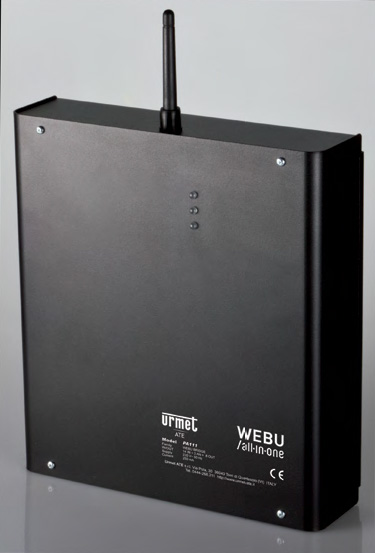
\includegraphics[width= 0.5\linewidth]{pictures/webuall.png}
	\caption{Foto di una Webu All-In-One}\label{fig:webuall}
\end{figure}
LIS sfrutta una serie di tecnologie innovative in tutti i settori del controllo di sicurezza, si parte dall'installazione dell'hardware dal cliente che solitamente comprende una centrale antintrusione di ultima generazione tra cui:
\begin{itemize}
	\item Tecnoalarm
	\item UTC Fire \& Security
	\item Bentel
\end{itemize}
Tutte centrali che permettono la ricezione degli allarmi tramite connessioni ADSL e GPRS, ed inoltre forniscono dei software di telegestione tramite gli stessi canali di comunicazione.\\
Affiancato alla centrale antintrusione solitamente LIS installa una centrale di backup come ad esempio la \emph{Webu All-In-One} della \emph{Urmet} questa centrale viene utilizzata come backup della centrale di sicurezza avendo alcuni ingressi programmabili, inoltre viene utilizzata come ponte per il vettore PSTN. Infine, dove possibile, viene installato anche un sistema di videosorveglianza che permette un analisi più approfondita della situazione. In particolare, dove il budget lo permette, viene installato un sistema \emph{Dallmeier} che offre meccanismi di compressione delle registrazioni quando queste vengono consultate da remoto\cite{dallmeier:premote}.\\
Quanto visto fino ad ora è quello che LIS installa dal cliente; vediamo adesso, invece, come LIS riceve e gestisce gli allarmi. In primo luogo, prima del nostro intervento, LIS utilizzava solo i vettori PSTN, GSM e solo per alcuni modelli della \emph{UTC}, il vettore GPRS nonché per le periferiche di backup interne. Per ricevere gli allarmi su questi vettori utilizzavano due sistemi, il primo chiamato \emph{System III} è un sistema di ricezione allarmi su PSTN che permette di ricevere gli allarmi tramite il protocollo Contact-ID o SIA su PSTN e quindi su linea telefonica tradizionale tramite i toni. Il secondo sistema è chiamato Osborne Hoffman LAN che permette, tramite un protocollo proprietario, di ricevere gli allarmi sul canale GPRS per alcuni modelli della \emph{UTC Fire \& Security}.\\
Questi due ricevitori permettono la ricezione degli allarmi, tuttavia, per permettere la gestione di tali allarmi LIS sfrutta un programma proprietario denominato \emph{E-Pro} che permette la gestione degli allarmi presentando l'anagrafica del cliente, il posizionamento del sensore che è andato in allarme, una segnalazione esaustiva della tipologia di allarme ed altre informazioni che possono essere utili all'operatore, il quale una volta preso in carico una segnalazione la gestisce e compila un rapporto di gestione.
\begin{figure}
\centering
%\includegraphics[width=0.5\linewidth]{pictures/epro.png}
\caption{Schermata del software E-Pro}\label{fig:epro}
\end{figure}
\section{Cosa offre il mercato}
Al nostro arrivo in LIS la situazione presente era quella specificata in precedenza e quindi le centrali supportate erano molto poco ed inoltre il vettore di comunicazione principale era il PSTN. Si è quindi deciso di analizzare che cosa offrisse il mercato per valutare se sostituire il software E-Pro o aggiornarlo per renderlo più competitivo rispetto alla concorrenza.\\
Adesso analizzeremo quali sono i principali prodotti che avrebbero potuto sostituire il software di Lis analizzando in dettaglio i punti a favore e quelli a sfavore della scelta.
I software che analizzeremo sono:
\begin{itemize}
	\item AteArgo di Urmet
	\item WebSat Enterprise di AMA Software
	\item Advisor Managment di UTC Fire \& Security
	\item Mastermind e x-View di Enai
\end{itemize}
\subsection{AteArgo}
AteArgo è un prodotto che ha alle spalle vent'anni di sviluppo da parte di \emph{Urmet}, esso si basa su un sistema Unix/Linux ed è stato il primo software per vigilanze private creato in Italia. Il continuo confronto con il mercato e l'aggiornamento tecnico costante anno permesso di perfezionare sempre più AteArgo e adattarlo alle reali esigenze delle centrali operative degli istituti di vigilanza.\\
La centrale AteArgo è composta da due server uno principale e uno di backup con allineamento automatico dei dati in maniera trasparente all'operatore. Il software è multi-operatore e multi protocollo e prevede di base la gestione dei teleallarmi radio, PSTN e GSM, inoltre per le centrali Urmet permette anche la ricezione degli allarmi tramite vettori GPRS e TCP/IP. Il software permette di gestire delle periferiche mobili GPS per applicazioni di teleallarme come l'invio della pattuglia più vicina in caso di allarme o la verifica del servizio di ronda. Nell'ultima versione del software è possibile, tramite l'ausilio di periferiche aggiuntive, l'acquisizione video automatica dalle centrale AteArgo a seguito di un evento di allarme. Infine è possibile la gestione di sistemi video navigabili via browser.\\
Oltre a queste funzionalità il sistema è in grado di eseguire alcune funzioni automatizzate come effettuare chiamate automatiche per particolari segnalazioni effettuare il backup a caldo sia della centrale principale che quella di riserva, invio di segnalazioni direttamente al cliente tramite SMS, gestione automatica di un call-center e di un agenda cliente.\\
AteArgo fornisce anche la possibilità di rilevazioni statistiche sia in formato elettronico sia via Web. possibilità di creare report personalizzati o l'interazione con altri sistemi di centralizzazione.\\
Per quanto riguarda la gestione multi operatore ad ogni operatore viene assegnato un profilo specifico in base al suo livello di specializzazione. Per accedere al sistema ogni operatore si identifica tramite login e password con le quali attiva le funzioni a lui destinate.\\
L'interfaccia utente permette di intervenire all'arrivo di un allarme con il minor numero di azioni. Inoltre vi è un costante monitoraggio del sistema e dei collegamenti periferici.\\
Oltre a queste funzionalità di base il sistema può essere espanso tramite moduli software aggiuntivi tra cui:
\begin{itemize}
	\item comunication server: il sistema permette la comunicazione con altri sistemi informativi in modo bidirezionale assumendo la funzionalità di front-end.
	\item Utente ricaricabile: consente alla vigilanza di gestire clienti di tipo "ricaricabile" ovvero con la possibilità da parte del cliente di attivare o disattivare il servizio di vigilanza solamente tramite l'invio di un SMS.
	\item Verbali: garantisce la rintracciabilità di tutte le azioni della centrale operativa e legate ad un allarme e supporta l'operatore nella gestione degli eventi.
	\item ArgoSound: permette la gestione di determinate segnalazioni tramite una chiamata vocale automatica.
	\item Fast call: compone automaticamente un numero dalla lista dei contatti del cliente in allarme evitando errori o perdite di tempo.
	\item Messaging: permette alla centrale di inviare automaticamente SMS, FAX o E-Mail verso recapiti preimpostati nel caso di particolari eventi.
	\item Modulo database: relaziona e rende disponibili tutti i dati archiviati e permette di eseguire qualsiasi tipo di ricerca, inoltre permette di interfacciarsi con altri sistemi. Permette la creazione di indici per la stima e la valutazione degli interventi.
	\item  Modulo installatore: questo modulo permette di sollevare l'operatore dal supervisionare una nuova installazione dando la possibilità al tecnico di collegarsi alla centrale mediante portatile o smartphone e verificare la corretta ricezione degli allarmi dell'impianto sul quale sta intervenendo.
	\item Modulo GPS: permette di ricevere in centrale la posizione in tempo reale del parco pattuglie e di inviare sul sito in allarme la pattuglia più vicina.
	\item Modulo video: permette alla postazioni operatore di collegarsi a video server e telecamere IP in tempo reale.
\end{itemize}
\subsection{WebSat Enterprise}
WebSat Enterprase è un software sviluppato da AMA per la gestione di problemi di sicurezza ed emergenza degli ambienti, delle persone e dei veicoli. Esso consente la gestione di diverse tipologie di dispositivi di teleallarme come combinatori telefonici digitali (Contact ID, SIA, Fast Format), combinatori telefonici a sintesi vocale, teleallarmi radio. Inoltre tramite l'ausilio di periferiche AMA è possibile la gestione di teleallarmi via GSM/GPRS o IP, video allarmi, video sorveglianza con telecamere IP ed anche localizzazione satellitari per il controllo delle pattuglie, dei furgoni per il trasporto valori e qualsiasi tipo di veicolo.\\
Oltre a queste caratteristiche il software \emph{WebSat Enterprise} permette un'interazione automatizzata verso il cliente tramite SMS o chiamate pre-registrate. Gestisce, inoltre, i servizi di pattuglia e di ronda tramite il sistema di localizzazione satellitare. Infine permette la gestione della videosorveglianza.\\
Per quanto riguarda l'aspetto amministrativo il software permette l'integrazione con i software amministrativi e gestionali già presenti in azienda ed è  possibile predisporre un interfacciamento per la ricezione di allarmi provenienti da altri software.\\
Il software WebSat Enterprise è:
\begin{description}
	\item [Multifunzionale:] in quanto permette all'operatore di gestire tramite un unica interfaccia sia gli allarmi provenienti da periferiche mobili sia da impianti di allarme fissi.
	\item [Geo-referenziato:] per ogni tipo di allarme sia esso fisso o mobile, vengono messe a disposizione dell'operatore il maggior numero di informazioni possibili.
	\item [Gestione delle pattuglie:] Tramite la periferica WebSat Patrol la centrale permette di gestire in modo automatizzato le pattuglie in modo da ottimizzare le pattuglie sul territorio.
	\item[Report di comunicazione verso i clienti:] la centrale è in grado di inviare avvisi di stato di allarme in modo automatico via SMS , invio automatico di report mensili, possibilità da parte del cliente di richiedere report parziali tramite l'invio di SMS.
	\item [Interfacciamento automatico con centralino telefonico:] WebSat Enterprasie consente l'automazione delle chiamate verso i contatti telefonici del cliente in caso di allarme.
	\item[Interfacciamento con altri ricevitori:] oltre ai ricevitori di AMA la Websat enterprise è in grado di interfacciarsi con tutti i ricevitori telefonici che implementano i protocolli ADEMCO 685, standard SurGuard, per ricevere gli allarmi in codice Contact ID, SIA level 2 e Ademco high Speed.
	\item [Ricezione allarmi da combinatori con sintesi vocale:] la centrale di AMA è in grado di ricevere allarmi tramite chiamate effettuate da combinatori telefonici con sintesi vocale, solamente assicurandosi che il numero del chiamante sia in chiaro.
	\item [Gestione telecamere Axis:] ad ogni sistema di teleallarme è possibile combinare una o più telecamere Axis con connessione diretta via Internet in modo da mettere a disposizione dell'operatore un sistema di videosorveglianza ad un costo contenuto.
	\item [Polling GPRS:] per quelle periferiche che sono connesse tramite canale GPRS o TCP/IP la centrale è in grado di effettuare un polling ad intervalli molto brevi per verificare l'esistenza in vita della periferica e rilevare in modo tempestivo eventuali problemi di connessione.
\end{description}
\subsection{Advisor Managment}
Advisor Managment è una soluzione di UTC Fire \& Security pensata per centralizzare la gestione della sicurezza di uno o più siti facenti riferimento ad un unica centrale di sicurezza. Tuttavia questo prodotto non è pensato specificatamente per le vigilanze bensì per piccoli complessi residenziali o commerciali aventi un unica centrale di monitoraggio.\\
Questo sistema si concentra sulle caratteristiche necessarie alla gestione della sicurezza in ambienti particolari nel quale accedono dipendenti e lavoratori, nel quale si hanno orari di lavoro flessibili. Solo la gestione integrata di controllo accessi, sicurezza antincendio e videosorveglianza permette ai security manager di avere una visione chiara e completa di tutto il sistema.\\
L'advisor managment offre un interfaccia intuitiva per la gestione di ambienti differenti, un'unica interfaccia per funzioni multiple, consente la creazione di report e rivolto alla gestione efficiente degli allarmi qualunque essi siano.\\
Per quanto riguarda la videosorveglianza l'advisor managment è in grado di supportare tutti i videoregistratori di rete TrueVison, questa integrazione permette agli operatori di avere accesso sia alle telecamere in tempo reale sia agli eventi registrati consentendo così una verifica immediata degli eventi di allarme.\\ 
L'advisor management supporta le centrali antintrusione della linea advisor management e advisor advance questo permette una gestione combinata di sistemi antintrusione e di videosorveglianza, inoltre è possibile configurare aree ad accesso limitato. Nel caso di rilevazione di un allarme, questo viene evidenziato nell'area di competenza e le immagini vengono mostrate in modo automatico all'operatore. Advisor management permette inoltre l'integrazione con le centrali di rilevazioni incendi della serie FP sia per il monitoraggio degli eventi sia per tutto quello che riguarda la gestione dell'impianto. Tutto questo integrato in un unico software permette di intervenire in modo tempestivo in caso di incendio; infatti, in caso di allarme la posizione del sensore viene mostrata dinamicamente e viene attivato il flusso video in tempo reale per verificare la presenza dell'incendio. Inoltre, grazie al sistema di controllo accessi è possibile sbloccare tutte le porte in modo automatico, e gli ascensori portati a terra.
\subsection{Mastermind e X-View}
Mastermind è uno dei prodotti più utilizzati dalle maggiori industrie di sicurezza principalmente in US ma ultimamente anche nel resto del mondo sia nel settore privato che in quello pubblico. Questa diffusione è dovuta alla grande sicurezza e affidabilità del sistema unita alla possibilità di gestire sistemi su larga scala. I punti di forza di mastermind sono la possibilità di lavorare sia con ambienti di piccola scala sia con ambienti più grandi. Possibilità di configurazione multi sito con ridondanza a caldo. Integrazione di molti sistemi in un unica interfaccia di sistema.\\
Mastermind è un sistema ad architettura aperta per fare in modo che i compratori possano adattare le loro tecnologie al sistema; esso permette la comunicazione tramite rete locale LAN e mette a disposizione degli SDKs per supportare al meglio lo sviluppo da parte di venditori di terze parti. come vendor di videosorveglianza.\\
Il sistema si suddivide in due parti slegate, una parte tratta il monitoring degli allarmi, l'altra parte, denominata \emph{business suite} si occupa del contatto e della gestione del cliente. Tutte queste funzioni sono supportate da una serie di applicazioni che permettono una gestione ottimale del sistema come il MASVideo che permette di registrare sui server le immagini associate ad un allarme o il MASWeb utilizzato per consentire un accesso remoto alla reportistica a clienti con particolari esigenze. Oppure X-View un software affiancato a MasterMind che permette all'operatore di costruire la propria interfaccia personale e mette a disposizione maggiori informazioni come la localizzazione GPS o la piantina dell'edificio.\\
A differenza degli altri prodotti analizzati mastermind risponde alle esigenze impostate dal cliente tramite l'utilizzo di workflows che gestiscono tutti gli eventi in modo tale da guidare l'operatore lungo una sequenza predefinita di operazioni. Inoltre questo meccanismo permette di gestire in modo automatico le operazioni più semplici e che non richiedono la necessità dell'interazione con l'operatore.\\
La parte di \emph{business suite} comprende tre sotto sezioni, la prima per definire le promozioni ed i prezzi da applicare ai clienti e organizza gli appuntamenti per le vendite. La seconda parte si occupa della relazione col cliente contenendo i dati del contratto la fatturazione dei servizi e il controllo dei pagamenti. l'ultima parte invece si occupa dell'organizzazione dell'installazione e dell'attivazione del servizio, si può occupare della gestione del magazzino mantenendo un inventario aggiornato.
Le funzionalità di Mastermind sono:
\begin{description}
	\item[VRT/IVR] ovvero la possibilità di sfruttare un centralino automatico che risponde alle richieste più comuni dei clienti senza tenere occupato inutilmente un operatore di centrale, inoltre questa funzionalità può essere sfruttata per creare chiamate automatizzate verso il cliente nel caso di allarmi specifici.
	\item[Voice Recorder Integration:] tutte le chiamate in entrata ed in uscita possono essere registrate e immagazzinate per un successivo controllo sia da parte del cliente che da parte della vigilanza nel caso in cui sia necessaria una verifica.
	\item[Report Server:] questa funzionalità permette l'invio di email o messaggi periodici con il riassunto degli allarmi e degli interventi.
	\item[MASWeb:] questa funzionalità permette ai clienti e ai tecnici di accedere alle loro informazioni per generare report o modificare i dati. Le pagine web sono strutturate per includere i servizi di monitor e reportistica, l'elenco dei servizi e le informazioni di fatturazione. I tecnici possono modificare uno stato dell'impianto e inserirlo in modalità test per ricevere sul proprio browser o sull'app l'esito dei test effettuati durante una manutenzione o installazione.
	\item[MASmobile:] questa app permette di controllare lo stato del sistema effettuare controllare lo storico eventi, agli installatori permette di mettere il sistema in modalità test per ricevere gli esiti.
	\item[Controllo accessi:] è possibile integrare la ricezione degli allarmi con sistemi di controllo accessi 
\end{description}
\chapter{Obiettivi della tesi}
\label{capitolo3}
\thispagestyle{empty}

L'obiettivo di questa tesi è quello di illustrare le modifiche, le aggiunte ed i cambiamenti effettuati al software di LIS per permettere un integrazione dei ricevitori di allarme in maniera più veloce e standard, una seconda parte della tesi complementare alla prima si focalizza invece sulla telegestione del delle centrali di allarme. 
\section{La situazione iniziale}
Al nostro arrivo in LIS la situazione che si presentava era poco chiara e non ben definita. Gli operatori di centrale che gestivano gli allarmi utilizzavano un software denominato \emph{E-Pro}. Questo programma è un adattamento di un programma utilizzato da \emph{Cobra S.p.a} per la gestione degli allarmi provenienti da veicoli ed è stato adattato  negli anni alla gestione degli impianti fissi.\\
Questo software è un formato da un insieme di moduli alcuni scritti in C ed altri in Java, la parte che riguarda la ricezione degli allarmi il loro immagazzinamento nel database e la logica che gestisce il comportamento da intraprendere per la loro gestione è implementato in una serie di moduli scritti in C; questi moduli sono chiamati:
\begin{itemize}
	\item cp220\_4
	\item cp220\_3
	\item MTSfe\_fissi
\end{itemize}
Questi tre moduli si occupano della ricezione degli allarmi dai vettori PSTN e GPRS/GSM per fare questo utilizzano dei ricevitori fisici chiamati
\begin{description}
	\item[System III:] si occupa della ricezione degli allarmi sul vettore PSTN tramite protocollo Contact ID.
	\item[OHLan:] questo ricevitore è un PC fisico collegato nella rete locale sul quale è installato un software della UTC Fire \& Security che si occupa della ricezione tramite protocollo proprietario degli allarmi provenienti dalle centrali UTC.
	\item[Modem GSM:] più di un modem GSM è collegato ad una porta multi seriale connessa nella rete locale questi modem permettono la ricezione degli allarmi tramite vettore GSM e GPRS per quelle periferiche di backup di derivazione automotive.
\end{description}
Per quanto riguarda la parte Java essa si occupa dell'interazione con l'operatore e quindi il compito di questi moduli è quello di prelevare gli allarmi dal database e mostrarli all'operatore, inoltre,essi si occupano, anche, di tenere traccia di tutte le azioni eseguite dall'operatore. Questa parte è strutturata in modo da garantire la multiutenza, infatti, questi moduli sono scritti in Java EE e sono eseguiti su di un server JBoss in modo da permettere l'esecuzione di più sessioni contemporaneamente.
\begin{figure}
\centering
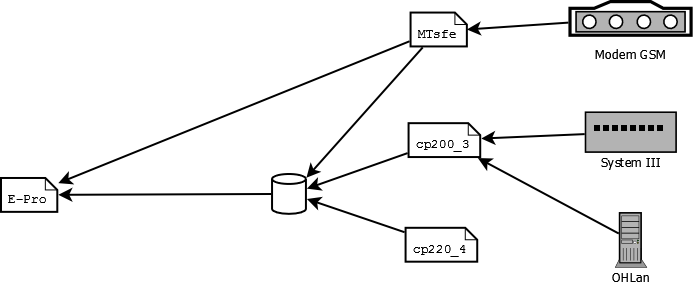
\includegraphics[width=0.9\linewidth]{pictures/struttura.png}
\caption{Schema dei moduli applicativi di LIS}\label{img:struttura}
\end{figure}
\subsection{cp220\_4}
Il \emph{cp220\_4} ha la funzione di leggere e trasformare gli allarmi provenienti dai sistemi di ricezione come il \emph{System III} o lo \emph{OHLan} e di immagazzinarli in un database non prima di averli trasformati in un formato interpretabile dall'E-Pro. Questo formato è derivato direttamente dal Contact ID il prevedere diversi campi
\begin{center}
	\texttt{ACCT MT QXYZ GG CCC S}
\end{center}
dove le diverse sigle indicano:
\begin{description}
	\item[ACCT:] è un identificativo assegnato al cliente
	\item[MT:] è un numero che indica il tipo di messaggio, se esso è nuovo oppure una ritrasmissione.
	\item[XYZ:] è un codice che indica il tipo di evento che è avvenuto
	\item[Q:] un numero che può essere 1 o 3 ed indica se l'evento trasmesso è rispettivamente iniziato o finito.
	\item[GG:] è il numero che identifica la partizione nella quale è stato generato l'allarme
	\item[CCC:] è un numero che identifica il sensore o zona che ha generato l'allarme.
	\item[S:] valore di checksum per il controllo degli errori
\end{description}
Il \texttt{cp220\_4} utilizza i campi ACCT, XYZ, Q, GG, CCC insieme al all'orario nel quale arriva il messaggio e li inserisce in una tabella del database dal quale poi saranno prelevati ed inviati all'operatore.\\
Oltre a questa funzione il modulo all'arrivo di ogni messaggio aggiorna un campo in una tabella chiamata \texttt{seriale} utilizzata controllare periodicamente lo stato in vita dei ricevitori e la loro connessione con il modulo in questione.\\
Questo modulo è il più interessante per noi in quanto è quello che permette la ricezione degli allarmi e quindi il modulo sul quale ci concentreremo per sviluppare la nostra applicazione di ricezione; in realtà esso ci servirà per comprendere la logica che un ricevitore deve eseguire una volta ricevuto l'allarme.
\subsection{cp220\_3}
Questo modulo si occupa della logica della gestione degli allarmi per capire meglio il funzionamento di questo modulo facciamo un esempio e consideriamo un locale commerciale con prefissati orari di apertura e di chiusura. Il sistema di allarme viene disinserito poco prima dell'apertura, in questo caso alla centrale arriva l'evento di disinserimento dell'impianto ma il cp220\_3 controlla l'orario di arrivo di tale evento e calcola che questa segnalazione è conforme all'orario di apertura e quindi lo registra ma non lo inoltra agli operatori di centrale. Nel caso in cui, invece, tale evento di disinserimento si verifica durante le ore notturne, e quindi fuori dal normale orario di apertura allora il software verifica l'anomalia e invia la segnalazione all'operatore che provvederà a gestirla.\\
Il \texttt{cp220\_3} si occupa di capire quali segnalazioni inviare all'operatore. Oltre al controllo orario visto in precedenza, si occupa di filtrare le segnalazioni multiple provenienti ad esempio da ritrasmissioni, di filtrare gli impianti in test o disattivati che comunque inviano segnalazioni alla centrale.
\subsection{MTSfe}
Lo \texttt{MTSfe} è un software che deriva da \emph{Cobra Italia} e si occupa principalmente della gestione delle periferiche di backup di derivazione automotive ovvero delle periferiche \emph{PowerSat}. Queste periferiche erano state pensate per il controllo di autoveicoli e sono state adattate all'utilizzo negli impianti fissi come periferiche di backup in quanto sono dotate di una decina di ingressi programmabili e di alcune contatti di uscita.\\
Questo modulo pur essendo rimasto parte integrante del software di LIS è ancora di proprietà di Cobra Italia è perciò stato impossibile per noi modificarlo, tuttavia uno dei nostri obiettivi a lungo termine era quello di sostituire le vecchie periferiche di backup PowerSat con altre più preformanti e aperte così da poter essere gestite direttamente dal nuovo software.
\subsection{E-Pro}
\emph{E-Pro} è il software centrale che gestisce l'interazione tra operatore e sistema. Mentre i moduli in C si occupano di ricevere e selezionare gli allarmi il software E-Pro si preoccupa di prelevarli dal database e mostrarli all'operatore per poi aiutarlo nella gestione e controllo della segnalazione.\\
Questo software è composto da una serie di moduli Java EE che vengono eseguiti in un ambiente JBoss. Questi moduli hanno compiti diversi e svolgono le diverse funzionalità tra cui:
\begin{itemize}
	\item autenticazione e profilazione degli utenti che utilizzano E-Pro;
	\item gestione dell'interfaccia grafica;
	\item elaborazione finale degli allarmi;
	\item gestione della reportistica.
\end{itemize}
\section{Obiettivi della tesi}
Gli obiettivi di questa tesi sono diversi e intervengono su diversi aspetti del software preesistente ma tutti questi obiettivi si prefiggono lo scopo principale di strutturare il software in maniera adeguata per permettere l'estensione delle funzionalità in modo rapido e strutturato permettendo così in futuro di non dover ripensare e riscrivere il software per integrare nuovi protocolli o aggiungere nuove funzionalità al software.
\subsection{Integrazione di nuovi protocolli in minor tempo}
Il primo degli obiettivi che vogliamo analizzare è quello dell'integrazione dei nuovi protocolli. Per prima cosa dobbiamo fare una piccola distinzione in due casi il primo caso si ha quando le segnalazioni di allarme arrivano da un ricevitore esterno come avveniva in precedenza con il System III  in questo caso il protocollo da integrare è quello del ricevitore che si interpone tra la centrale di allarme ed il software di ricezione. Il secondo caso si ha quando la centrale d'allarme comunica direttamente con il software di ricezione.  I due casi se pur distinti sono simili in quanto si può trattare il ricevitore esterno come una centrale d'allarme che comunica gli eventi con identificativi diversi.\\
Per fare ciò si è pensato di sostituire o comunque affiancare al cp200\_4 un nuovo modulo che memorizza gli allarmi sulla base di dati nello stesso modo del cp200\_4 per mantenere la retro compatibilità del software. Questa soluzione è stata una scelta obbligata per non dover riscrivere interamente il software tuttavia, come vedremo nella sezione successiva, non è stata una scelta ottimale.
\subsection{Strutturazione del software}
Il secondo obiettivo che ci siamo prefissati è stato quello di dare al software una struttura più solida e modulare in modo da non dover riprogettare il software in futuro con la richiesta di nuove funzionalità come è stato necessario nel nostro caso. Per fare ciò si è deciso di strutturare anche la parte C in un software ad oggetti con conseguente passaggio obbligato al linguaggio C++. La scelta del linguaggio C++ rispetto al Java è stata una scelta puramente pratica in quanto le nostre conoscenze erano più sbilanciate verso questo linguaggio inoltre, la gestione delle periferiche seriali è più semplice utilizzando tale linguaggio.
\subsection{Telegestione}
Una funzione completamente nuova richiesta dalla centrale operativa era quella di poter telegestire le diverse centrali direttamente dal software E-Pro. Per fare ciò è stato necessario innanzitutto capire quali erano le funzioni necessarie per una corretta telegestione da parte dell'operatore. In secondo luogo è stato necessario capire quali centrali fossero in grado di permettere tali funzionalità e su quale vettore di comunicazione erano disponibili. Infine a livello pratico è stato necessario capire in quale modo implementare tali funzioni.\\
Obiettivi secondari alla telegestione sono stati la minimizzazione dei tempi di reazione del software e lo studio di una nuova interfaccia grafica per esprimere in modo immediato le nuove informazioni messe a disposizione dell'operatore.
\subsection{Utilizzo di nuovi vettori di comunicazione}
Gli obiettivi di rinnovamento del software non potevano limitarsi solamente ad un nuovo software ma, soprattutto, erano legati in modo indissolubile dall'utilizzo di nuovi vettori di comunicazione in particolare TCP/IP, GPRS ed SMS per minimizzare i costi di comunicazione e diminuire i tempi di dialogo tra la centrale di allarme e la centrale operativa.\\
L'utilizzo di questi vettori ha comportato lo studio di protocolli specifici come il Contact-ID o il SIA over IP e l'utilizzo e quindi l'interfacciamento del software con nuovo hardware come i modem GPRS.
\section{Vincoli di progetto}
Con il nostro arrivo sono state introdotte numerose modifiche al software preesistente tuttavia per mantenere l'operatività e l'usabilità durante tutto lo sviluppo è stato necessario effettuare alcune scelte che permettessero la retro compatibilità e la normale esecuzione del software preesistente. In particolare è stato necessario mantenere il meccanismo nel quale il cp220\_4 memorizzava gli allarmi nel database. Questo memorizzazione consisteva nell'inserimento in tabella di un nuovo record composto da diversi campi tra cui il codice della centrale, il codice di allarme, il numero della partizione, della zona, la data e l'ora in cui è avvenuto l'evento e altre informazioni che saranno mostrate in dettaglio nel \chaptername~\ref{capitolo4}.\\
Questo meccanismo tuttavia porta con se diversi problemi.
Il primo problema che si presenta anche se di facile soluzione si ha quando la segnalazione di allarme non porta con se l'ora della segnalazione, questo problema si risolve impostando l'ora della ricezione come ora in cui è avvenuta la segnalazione, tuttavia questo tipo di informazione è superflua in quanto non viene utilizzata in nessuna altra parte del software.\\
Il secondo problema più complesso consiste nel codice di allarme, esso è simile al Contact ID tuttavia, il Contact ID ha una struttura \texttt{QXYZ} dove Q è uno tra i numeri 1, 3 o 5 che indicano rispettivamente il nuovo evento, il termine di un evento e la continuazione di una segnalazione mentre XYZ è un codice identificativo del tipo di evento. mentre la memorizzazione avviene con un codice che ha la forma \texttt{XYZQ} ovvero con il numero rappresentato dalla lettera \texttt{Q} in coda rispetto al Contact ID standard questo comporta delle elaborazioni aggiuntive prima di memorizzare il dato. Inoltre il codice Contact ID non è completamente univoco ma per alcune segnalazioni su centrali differenti avremmo significati diversi questo, in precedenza era stato risolto con una tabella nel database che associava ad un determinato tipo di centrale le corrispondenti etichette con il significato del codice. Questo meccanismo è rimasto invariato tuttavia esso comporta che ad ogni integrazione è necessario aggiungere centinaia di record a questa tabella per poter permettere la conversione. L'ultimo problema riscontrato riguardo l'adozione di questo tipo di memorizzazione è stato il fatto che non tutte le centrali comunicano tramite protocollo Contact ID e questo ha comportato l'introduzione di una tabella di traduzione per convertire i codici provenienti da altri protocolli in codici Contact ID.\\
Un problema che abbiamo riscontrato sempre riguardante i codici Contact ID riguardava il valore del campo \texttt{Q} in quanto questo campo è utilizzato dal cp220\_3 per effettuare il controllo orario di un impianto i codici 1401 e 3401 indicano rispettivamente l'inserimento ed il disinserimento da parte dell'utente dell'impianto, il cp220\_3 sfrutta questi due codici per verificare che tali eventi avvengano nelle fasce orarie prestabilite. Questo meccanismo funzionava correttamente per le centrali già integrate in quanto esse rispettavano questi codici per indicare gli inserimenti e i disinserimenti, tuttavia, per alcune centrali integrate durante il nostro percorso ci è capitato di trovarne alcune che invertivano i due codici e questo ci ha obbligati ad utilizzare la tabella di traduzione per mantenere un comportamento corretto del software.\\
Il principale problema riscontrato tuttavia nell'utilizzo del codice precedente è stato proprio la comprensione del suddetto codice sorgente mal commentato, con refusi  di vecchie funzioni provenienti da versioni precedenti e soprattutto la mancanza di una struttura logica del programma, basti pensare che il cp220\_3 e il cp220\_4 sono due programmi che svolgono due funzioni completamente distinte ma che in realtà provengono dallo stesso codice sorgente compilato con parametri differenti. Per ovviare a questo problema abbiamo innanzitutto introdotto il codice in un sistema di controllo versione, eliminato oltre diecimila righe di codice inutilizzato e commentato ogni singola funzione tramite un sistema di generazione della documentazione automatica. Questo ci ha permesso di comprendere le funzionalità del software anche se in alcuni casi non è servito a capirne il reale funzionamento o la logica con la quale è stato programmato; questo non ha causato grosse difficoltà ma potrebbe crearne quando si cercherà di sostituire il cp220\_3 con un nuovo modulo meglio strutturato.



\chapter{Progettazione logica}
\label{capitolo4}
\thispagestyle{empty}
\section{Nuovi vettori di comunicazione: dal PSTN al TCP/IP}
\section{I protocolli di comunicazione}
\section{Strutturazione del software}
\subsection{Dal cp220\_3 al \emph{Ricevitori 2.0}}
\subsection{Il software di telegestione}

%\chapter{Telegestore}
\label{capitolo5}
\thispagestyle{empty}
In questo capitolo analizzeremo la realizzazione di un software pensato per inviare dei comandi alle centrali e alle periferiche che permettono la telegestione. In particolare in questo capitolo ci concentreremo sul software che gestisce  la comunicazione tra la centrale operativa e le diverse centrali sia come comunicazione diretta sia tramite l'utilizzo di ricevitori.\\
Nel capitolo successivo, invece, concentreremo la nostra analisi sul modulo che permette all'operatore di inviare i comandi al software che analizzeremo in questo capitolo.\\
In particolare questo software comunicherà con le centrali della marca \emph{Tecnoalarm} che permettono una connessione diretta per la telegestione tramite l'ausilio di un protocollo proprietario, il \emph{Tecno Out}. Inoltre, come accennato nel capitolo precedente, sfrutteremo il ricevitore AteArgo per inviare dei comandi anche alle periferiche Webu All-In-One.\\
Per quanto riguarda le funzionalità di questo software il suo scopo principale è quello di inviare comandi alle diverse periferiche, tuttavia per fornire maggiori informazioni all'operatore, ogni qualvolta che viene avviata la telegestione si richiedono alle periferiche ed alle centrali lo stato delle zone e delle partizioni in modo da avere sempre sotto controllo la situazione corrente.\\
\section{I protocolli di comunicazione}
Analizziamo ora come questo software comunicherà con le centrali, in particolare non ci addentreremo in dettaglio nei protocolli in quanto essi sono proprietari, ma analizzeremo la struttura del pacchetto e la comunicazione con la centrale o con il ricevitore interessato. In particolare analizzeremo i pacchetti di controllo del protocollo AteArgo per l'invio di comandi tra questo software e il corrispettivo ricevitore, e il protocollo \emph{Tecno Out} per la comunicazione con le centrali Tecnoalarm.
\subsection{Protocollo Tecno Out}
Il protocollo Tecno Out è un protocollo chiuso di proprietà di Tecnoalarm studiato per la comunicazione tra le centrali e sistemi di gestione remota come software di domotica o, come nel nostro caso, sistemi di telegestione.
\subsubsection{La struttura del pacchetto}
Pur non potendo addentrarci in particolare nella struttura del pacchetto analizzeremo alcuni punti salienti. Questo protocollo è orientato al byte e più in particolare il pacchetto ha una struttura molto semplice, il pacchetto è così costruito:
$$
\begin{array}{c}
\langle STX\rangle\langle codice\rangle\langle comando\rangle\langle len\rangle\langle dati\rangle\langle CRC16\rangle\\
\end{array}	 
$$
I diversi campi sono rispettivamente:
\begin{description}
	\item[STX:] campo composto da un unico byte e che delimita l'inizio del pacchetto;
	\item[codice:] questo campo è composto da 3 byte e contiene il codice utente per permettere l'accesso alla centrale
	\item[comando:] campo composta da un unico byte che identifica il comando da eseguire sulla centrale;
	\item[len:] indica la lunghezza del campo dati, essa varia in base al tipo di operazione da eseguire sulla centrale;
	\item[dati:] questo campo contiene le informazioni aggiuntive da utilizzare insieme al campo \emph{comando};
	\item[CRC16:] questo è il campo di controllo errori che sfrutta un algoritmo di CRC a 16 bit calcolato sul resto del pacchetto. Questo campo ha una lunghezza di due byte.
\end{description}
\subsubsection{La criptazione del pacchetto}
Questo protocollo sfrutta la criptazione AES a 128 bit. Ogni attore della comunicazione deve conoscere una chiave denominata \emph{PassPhrase} la quale verrà utilizzata insieme al vettore di inizializzazione.\\
Durante la prima fase il client invia un vettore di 17 byte contenete nei primi 16 byte il vettore di inizializzazione e nel diciassettesimo un valore predefinito criptato con il vettore appena inviato e con la PassPhrase. Il server quando riceve questo pacchetto salva i primi 16 byte come vettore e decripta il diciassettesimo con tale vettore e con la PassPhrase se il diciassettesimo byte decriptato corrisponde con il valore predefinito allora l'inizializzazione si conclude con successo e tutti i pacchetti successivi saranno criptati con tale vettore. In caso contrario il client chiude la connessione e riprova.\\
Non ci soffermeremmo oltre sulla criptazione in quanto nel codice questa operazione sarà effettuata da una libreria esterna e non implementata direttamente.
\subsubsection{La connessione}
La connessione è una semplice connessione client server tramite protocollo TCP/IP nel quale il nostro software svolge la funzione di client e la centrale d'allarme svolge quella di server. Questo significa che la centrale risponderà alle nostre richieste e non invierà messaggi se non interrogata. Durante la telegestione uno dei requisiti è quello di conoscere lo stato delle zone e delle partizioni perciò è necessario effettuare un polling per richiedere continuamente questi stati, ed all'inizio di ogni ciclo si controlla la presenza di nuovi comandi in coda.
In \fname{fig:contecno} vediamo come avviene la comunicazione, dopo la prima fase di inizializzazione del vettore di criptazione si prosegue con il ciclo di polling fino alla chiusura della connessione.
\begin{figure}
\centering
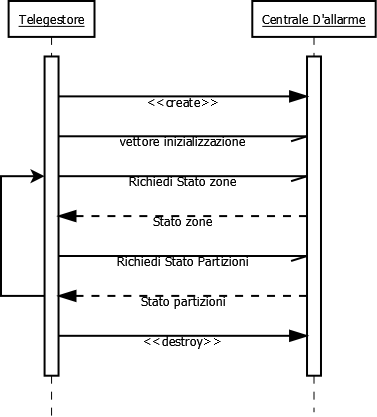
\includegraphics[width=0.7\linewidth]{pictures/contecno.png}
\caption{Scambio di messaggi tra software e centrali Tecnoalarm}\label{fig:contecno}	
\end{figure}
\subsubsection{I tipi di pacchetto}
In questo protocollo possiamo distinguere tre tipologie di pacchetto che sono:
\begin{itemize}
	\item messaggi di monitoring;
	\item messaggi di pilotaggio;
	\item messaggi di risposta.
\end{itemize}
I messaggi di monitoring servono per richiedere alla centrale di fornire informazioni riguardo al suo stato e a quello delle sue zone, i messaggi di pilotaggio sono quelli inviati dal nostro software verso la centrale per farle eseguire delle operazioni, infine, i messaggi di risposta sono quelli inviati dalla centrale per rispondere alle nostre richieste.
\paragraph{Messaggi di monitoring}
I messaggi di monitoring sono quei messaggi che il nostro software dovrà inviare alla centrale per richiedere lo stato di alcuni elementi, in particolare a noi interessa richiedere lo stato dei seguenti elementi:
\begin{itemize}
	\item lo stato delle zone;
	\item lo stato delle partizioni;
	\item lo stato della centrale;
	\item lo stato dei programmatori orari.
\end{itemize}
Per stato delle zone noi intendiamo se il singolo sensore è escluso, incluso oppure in allarme. Lo stato delle partizioni comporta sapere se esse sono inserite o disinserite o inserite solo in modo parziale. Per quanto riguarda le informazioni da conoscere sulla centrale, quelle che interessano a noi sono lo stato dell'alimentazione elettrica, quello della batteria e quello del tamper. Mentre l'unica informazione necessaria per i programmatori orari è se essi sono bloccati o in funzione.\\
Per reperire queste informazioni è necessario inviare alla centrale d'allarme il pacchetto formattato come precedentemente descritto con all'interno del campo codice un numero che ne identifica il comando. La centrale risponderà a questo comando inviando nel campo dati del pacchetto di risposta le informazioni. Prendendo come esempio le informazioni riguardanti la centrale noi inviamo il pacchetto specifico per richiedere queste informazioni e la centrale risponderà con un pacchetto con un unico byte nel campo dati. A questo byte deve essere applicata una maschera in AND per estrapolare le tre informazioni di cui necessitiamo.
\paragraph{Messaggi di pilotaggio}
I messaggi di pilotaggio servono per far eseguire delle azioni alla centrale d'allarme, per inviare i comandi da eseguire si utilizzano il pacchetto formattato così come indicato in precedenza con l'utilizzo di  opportuni codici. A differenza dei comandi di monitoraggio il campo dati questa volta contiene i valori da impostare sull'elemento selezionato. Ad esempio volendo escludere un opportuno sensore si invia alla centrale di allarme un pacchetto con l'opportuno valore nel campo comando e nei dati si inserisce il numero di zona e l'operazione da eseguire.\\
I comandi che interessano a noi sono solamente tre e riguardano le operazioni più comuni che gli operatori svolgono sulle centrali, ovvero, l'inclusione e l'esclusione di una zona, l'inserimento o il disinserimento di una partizione, ed infine il blocco o lo sblocco di un programmatore orario.
\paragraph{Messaggi di risposta}
I messaggi di risposta sono quelli che la centrale di allarme invia al nostro software essi possono essere di tre tipi:
\begin{itemize}
	\item ACK: in questo caso nel campo dati sono presenti eventuali risposte al messaggio inviato dal software come lo stato degli elementi richiesti.
	\item NACK: questo messaggio si riceve quando la centrale d'allarme non è in grado di interpretare il messaggio appena ricevuto e quindi non è in grado di dare una risposta.
	\item BUSY: questo tipo di messaggio di risposta si ottiene quando la centrale di allarme non è in grado di soddisfare le richieste perché occupata a svolgere altre operazioni o a soddisfare richieste precedenti.
\end{itemize}
L'ultimo messaggio è da tenere molto in considerazione in quanto esso limita il tempo di polling per gli stati della centrale, il protocollo infatti specifica che le richieste devono essere inviate con un intervallo minimo di 500ms.
\subsection{Protocollo Urmet}
Questo protocollo è lo stesso del capitolo precedente, in questo caso però analizzeremo i pacchetti necessari a richiedere lo stato degli ingressi e delle uscite e quello utilizzato per inviare i comandi, infine, analizzeremo le risposte a questi pacchetti.
\subsubsection{La struttura del pacchetto}
La struttura è quella che abbiamo visto nel capitolo precedente, si tratta di un protocollo basato su stringhe che formano una struttura XML con un tag di apertura seguito da una parte di header nella quali sono contenuti ora e data della trasmissione del pacchetto. Nel corpo del pacchetto invece troviamo le informazioni vere e proprie che dipendono dal tipo di pacchetto.
\subsubsection{La connessione}
Come si è visto la connessione con il software AteArgo è una connessione di tipo locale client-server nel quale il software di Urmet ricopre il ruolo di server. Tuttavia, pur essendo esso un server non permette la connessione di molteplici client questo ha comportato una problematica in quanto la connessione è necessaria al software ricevitore per mantenere la ricezione degli allarmi. Questo ci ha obbligati a pensare ad un meccanismo veloce e sicuro per far si che il ricevitore potesse inviare i comandi generati dal telegestore. Il meccanismo adottato è stato quello di una connessione socket tra \texttt{Ricevitore} e \texttt{Telegestore}, il \texttt{Telegestore} invia una stringa ad un server che viene eseguito ogni volta che viene avviato il software di ricezione. Questo meccanismo permette una comunicazione più rapida di quella che si avrebbe inserendo il comando in una tabella del database. 
Inoltre, questo tipo di comunicazione è stata pensata con un meccanismo di \emph{reques-replay} ed è quindi piuttosto affidabile.\\
Come nel caso precedente si attua un meccanismo di polling per richiedere lo stato degli ingressi e delle uscite di una determinata centrale, tuttavia in questo caso il polling no può essere molto stringente in quanto il software AteArgo effettua ogni volta la connessione con la periferica e non la mantiene aperta.
\subsubsection{I tipi di pacchetto}
Come abbiamo detto i tipi di pacchetto necessari per permettere di implementare le funzionalità richieste sono tre:
\begin{itemize}
	\item pacchetto di richiesta degli stati;
	\item pacchetto di comunicazione degli stati;
	\item pacchetto di comando.
\end{itemize}
\paragraph{Pacchetti di richiesta}
In questo tipo di pacchetto abbiamo che l'attributo del campo body è di tipo \emph{INO} nel campo body è presente solo l'identificativo della periferica di cui si vogliono conoscere gli stati.
\paragraph{Pacchetti di comunicazione degli stati}
In questo tipo di pacchetto abbiamo che l'attributo del campo body è uguale a quello della richiesta degli stati. In questo campo dopo le normali informazioni per identificare la periferica si ha una serie di campi per ogni ingresso od uscita che ne stabiliscono se è un contatto d'ingresso oppure un contatto d'uscita, se esso è impostato in modalità \emph{''normalmente aperto''} oppure in modalità \emph{''normalmente chiuso''} ed infine lo stato del contatto.
\paragraph{Pacchetto di comando}
In questo caso il pacchetto di comando contiene nella parte body le informazioni per identificare la centrale su cui effettuare i comandi e i contatti da attivare o disattivare.
\subsection{Protocollo Telegestore-Ricevitore}
Come abbiamo visto nella paragrafo precedente per permettere una comunicazione veloce ed efficiente tra il telegestore e il ricevitore che invia i comandi si è deciso di instaurare una connessione socket di tipo \emph{request-reply} tra i due software.\\
I due software si scambiano dei messaggi basati sullo stesso protocollo interno pensato per la comunicazione tra il server JBoss e il software di telegestione che vedremo nel capitolo successivo. Tuttavia qui accenniamo ad alcuni aspetti di questo pseudo-protocollo.\\
I pacchetti non sono altro che stringhe contenenti diversi campi separati da un carattere \emph{'';''}. I messaggi scambiati tra il telegestore e il software di ricezione hanno il seguente formato:
\begin{center}
	\textit{ce\_id;COM;elemento;numero;comando}
\end{center}
dove \texttt{ce\_id} è il codice che identifica la centrale, \texttt{elemento} indica su quale elemento eseguire il comando se esso è una zona o una partizione. Il campo \texttt{numero} indica il numero dell'elemento sul quale eseguire e, infine, il campo \emph{comando} contiene un codice per indicare quale azione eseguire sull'elemento identificato. Mentre il ricevitore, una volta eseguito il comando rimanda il pacchetto con indietro con l'aggiunta di un campo dopo comando con \emph{OK} se il comando è andato a buon fine o con \texttt{KO} se il comando è fallito.
\subsection{Altri protocolli}
Mentre scriviamo sono in implementazione nuovi protocolli di telegestione, alcuni simili o comunque riconducibili a quelli già analizzati come il \emph{CEI-ABI} protocollo standard per la ricezione di allarmi e la gestione di centrali d'allarme. La particolarità di questo protocollo è che mantiene sempre aperta la connessione con la centrale. Questa particolarità comporta un meccanismo tipo quello adottato con urmet per inviare i comandi in quanto è possibile aprire un'unica connessione ed è necessaria per la ricezione degli eventi.\\
Una seconda tipologia di telegestione in fase di sviluppo invece si basa sull'invio alle centrali di SMS preformatati e la centrale d'allarme risponde contattando la centrale operativa ed inviando le informazione richieste tramite i normali canali di comunicazione. Per questo tipo di comunicazione non è prevista la verifica dell'invio del comando e la comunicazione avviene tramite dei modem GPRS collegati su porte seriali.
\section{La struttura dati}
Come abbiamo visto in questo caso la comunicazione tra i diversi software avviene completamente tramite lo scambio di messaggi su socket. Tuttavia per poter tener traccia delle operazioni eseguite e dei comandi andati a buon fine si è deciso comunque di memorizzare sul database i comandi ed il loro stato in modo tale che in caso di crash del sistema sia possibile risalire agli eventi andati a buon fine e di quelli rimasti in sospeso.\\
La tabella realizzata a tale scopo è quella in \lname{lst:tabcodici}
\begin{lstlisting}[language=SQL,caption=Tabella comandi,label=lst:tabcodici]
CREATE TABLE comandi (
    cd_id integer NOT NULL DEFAULT nextval(('"comandi_cd_id_seq"'::text)::regclass),
    cd_tipo_comand integer,
    cd_tipo_element integer,
    cd_num_element integer,
    cd_stato character(1) DEFAULT 'n'::character varying,
    cd_risposta integer DEFAULT 0,
    cd_centrale character varying(5),
    cd_codice_hw character varying(30),
    CONSTRAINT cd_comandi_id_pkey PRIMARY KEY (cd_id)
)
\end{lstlisting}
dove i campi sono autoesplicativi, il campo stato indica se il comando è stato preso in gestione dal telegestore mentre il campo risposta indica la risposta che esso comunica al server JBoss. I campi \texttt{cd\_element} e \texttt{cd\_command} sono rispettivamente i campi associati ai valori che vengono trasmessi nel protocollo tra server in ascolto sul software \texttt{Ricevitore} e \texttt{Telegestore}.
\section{Architettura e realizzazione del sistema}
Analizziamo ora come è stato realizzato il sistema in particolare ci concentreremo su quella parte di software progettato per comunicare con le centrali d'allarme o con i ricevitori. Per quanto riguarda il funzionamento del software esso è molto semplice riceve una segnalazione da software JBoss e inizializza un thread che comunica con la centrale o con il ricevitore. Questo thread richiede più o meno periodicamente gli stati delle zone, delle partizioni e della centrale e li confronta con quelli precedenti nel caso in cui  vi sia una variazione tra lo stato precedente e quello attuale notifica al thread principale la variazione ed esso provvederà a notificarlo al software eseguito sul server JBoss.\\
Una precisazione è da fare per quanto riguarda la distinzione tra periferiche di backup e centrali d'allarme, le prime sono meno potenti ed hanno meno ingressi e non hanno la possibilità di dividerli in partizioni, tuttavia si comportano esattamente come delle centrali d'allarme; le seconde invece presentano un numero di uscite minore e solitamente sono adibite a funzioni specifiche come il collegamento con sirene esterne e quindi non sono controllabili come nel caso delle periferiche. Per uniformare il software si è deciso di trattare le periferiche di backup come fossero delle centrali d'allarme adottando però come convenzione il fatto che le partizioni nelle periferiche di backup rappresentano le uscite mentre le zone ne rappresentano gli ingressi. Questo meccanismo ci permetterà di attivare le uscite di una periferica semplicemente dando il comando di inserimento di una partizione. 
\begin{figure}[p]
	\centering
	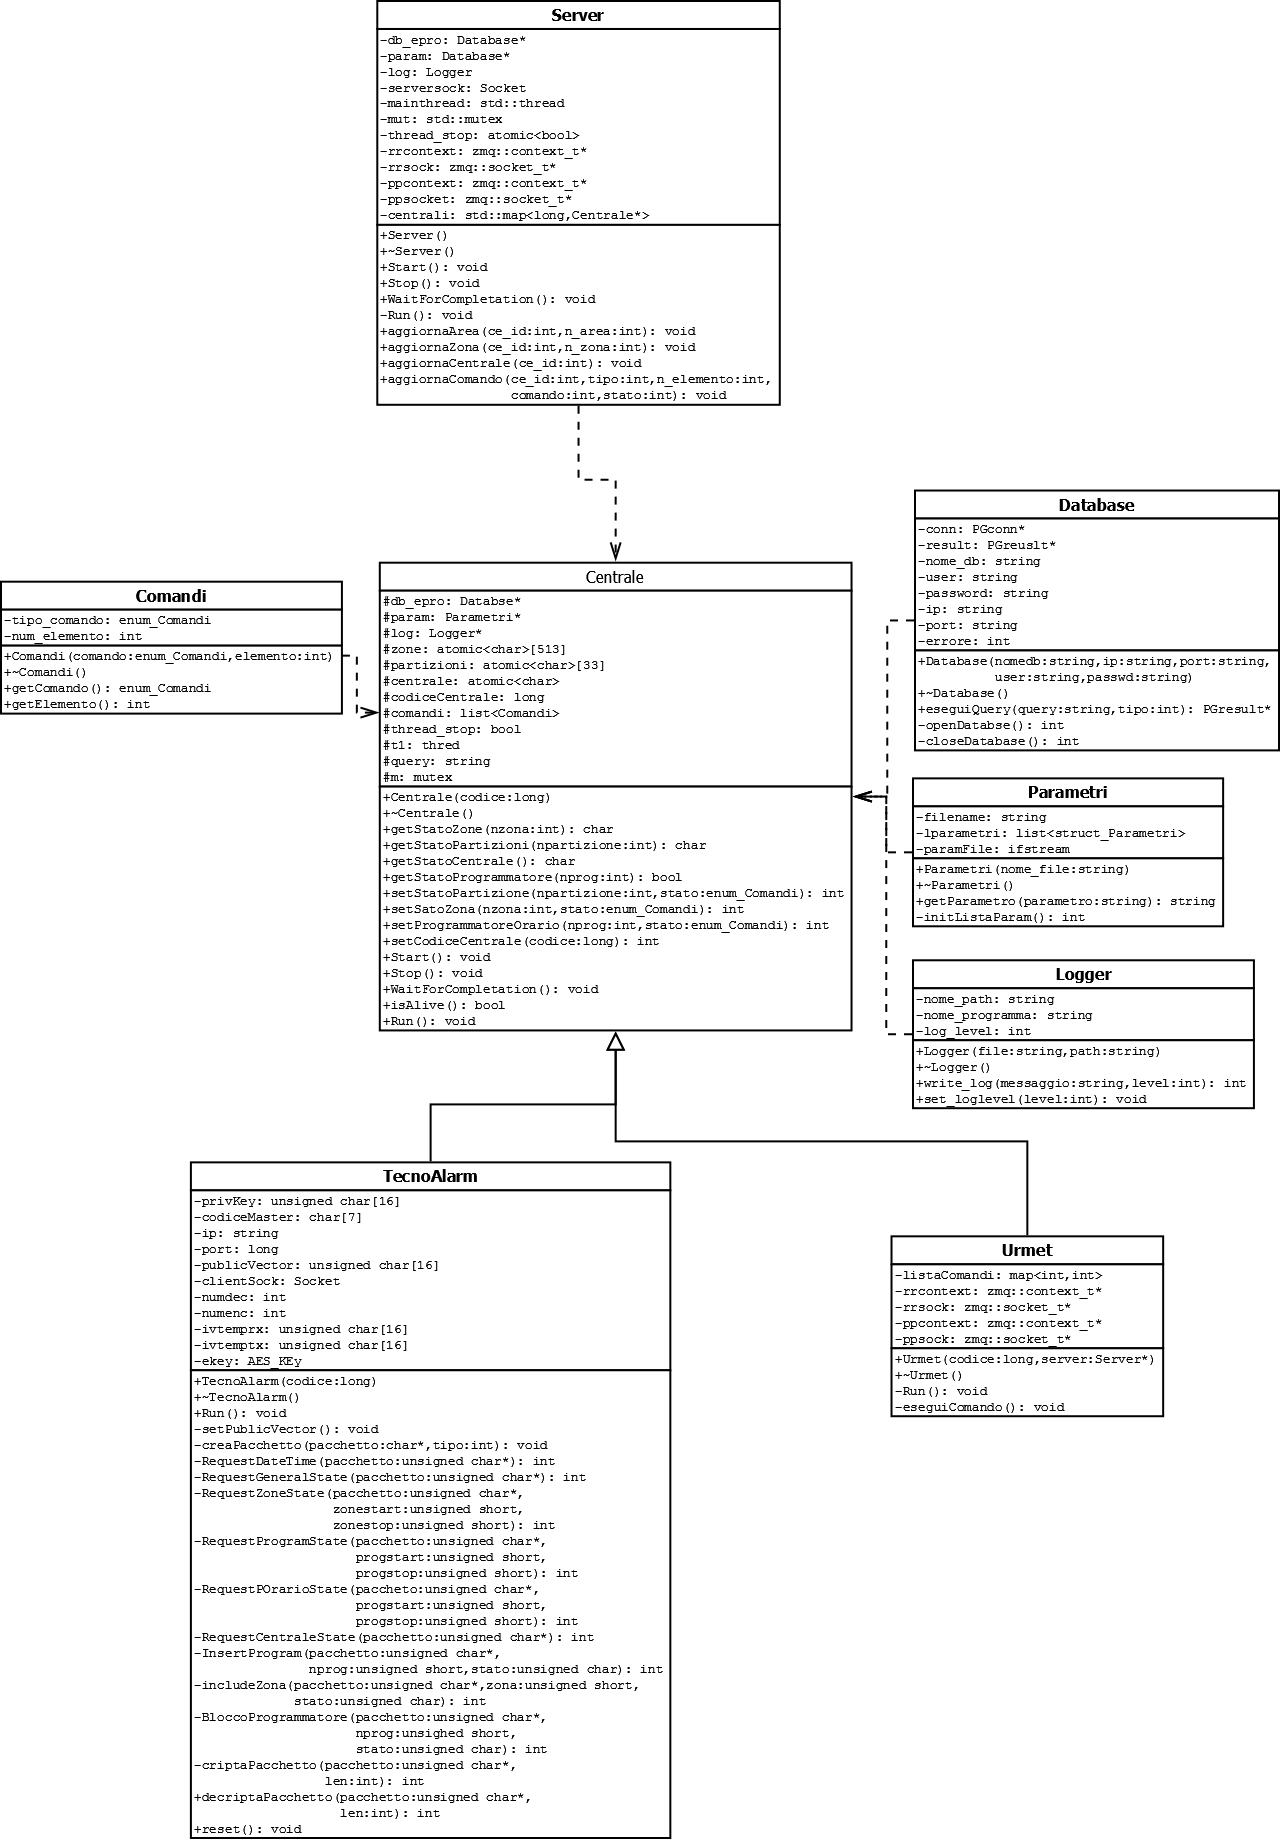
\includegraphics[width=\linewidth]{pictures/classitele.png}
	\caption{Schema delle classi del telegestore}\label{fig:classitele}
\end{figure}
\subsection{Le classi}
In \fname{fig:classitele} è mostrato lo schema delle classi del software. Analizziamo ora in dettaglio le diverse classi.
\subsubsection{Server}
Questa classe è la classe principale del software che gestisce la comunicazione con il software eseguito sul server JBoss. L'analisi di questa classe avverrà in maniera dettagliata nel prossimo capitolo.
\subsubsection{Centrale}
Questa classe è una classe astratta che serve da base per l'implementazione della telegestione delle diverse centrali di sicurezza. Essa prevede una serie di metodi per l'inserimento dei comandi in una \texttt{list<Comandi>} che poi sarà periodicamente controllata dal thread di esecuzione il quale preleverà il comando e lo eseguirà, questi metodi sono:
\begin{itemize}
\item \texttt{setStatoZona}
\item \texttt{setStatoPartizione}
\item \texttt{setStatoProgrammatoreOrario}
\end{itemize}
Oltre a questi metodi abbiamo una serie di metodi per prelevare l'ultimo stato memorizzato dei diversi elementi come lo stato delle zone, delle partizioni e della centrale, questi metodi sono:
\begin{itemize}
	\item \texttt{getStatoZona}
	\item \texttt{getStatoPartizione}
	\item \texttt{getStatoProgrammatoreOrario}
	\item \texttt{getStatoCentrale}
\end{itemize}
Essi restituiscono tutti come valore di ritorno un dato di tipo \texttt{char} dal quale si possono reperire tutte le informazioni riguardanti l'elemento richiesto semplicemente applicando una maschera in AND e valutando il valore dei singoli bit.\\
Il resto dei metodi servono per la gestione del thread principale, in particolare il metodo \texttt{Run()} è il metodo che deve essere implementato da tutte le classi che ereditano questa classe.
\subsubsection{Comandi}
Questa è una classe di supporto che memorizza il tipo di comando da eseguire e il numero dell'elemento sul quale eseguirlo.
\subsubsection{Tecnoalarm}
Questa classe implementa la telegestione per le centrali Tecnoalarm e ne implementa il protocollo. Essa estende la classe \texttt{Centrale} e ne implementa il metodo \texttt{Run}, questo metodo esegue il polling di richiesta degli stati richiedendo lo stato di tutte le zone e di tutte le partizioni e non solo di quelle attive; questo è possibile in quanto i tempi di comunicazioni sono molto ridotti. Quando viene rilevato un cambiamento rispetto ad uno stato precedente il thread utilizza l'attributo \texttt{Server} passato al costruttore per invocare i metodi \texttt{aggiornaArea}, \texttt{aggiornaZona} e \texttt{aggiornaPartizione} i quali creano ed inviano un messaggio ai moduli in esecuzione sul JBoss. Ad ogni ciclo, inoltre, il thread controlla che la lista dei comandi sia vuota, in caso non lo fosse preleva il primo comando della lista ed invia il comando alla centrale telegestita.\\
Gli altri metodi sono a supporto del metodo \texttt{Run} in particolare tutti i metodi esclusi \texttt{criptaPacchetto}, \texttt{decriptaPacchetto} e \texttt{reset} non fanno altro che riempire un array di caratteri con i valori necessari per creare un pacchetto valido secondo lo standard del protocollo, in particolare il metodo \texttt{creaPacchetto} riempie i campi comuni come il byte di start o il codice utente, gli altri metodi riempiono il campo dati e il campo codice in base ai valori passati dai parametri ed al tipo di metodo invocato. Il metodo \texttt{criptaPacchetto} serve per criptare il pacchetto prima dell'invio mentre il metodo \texttt{decriptaPacchetto} esegue l'operazione di decriptazione all'arrivo di un nuovo messaggio. Il metodo \texttt{reset} viene invocato nel caso in cui vi siano problemi di connessione o di decodifica dei messaggi, esso chiude la connessione resetta i valori di criptazione e reinizializza la connessione.
\subsubsection{Urmet}
Questa classe implementa la logica per la telegestione delle periferiche Urmet. Essa estende la classe \texttt{Centrale} e ne implementa il metodo \texttt{Run}; questo metodo in realtà non implementa il vero e proprio protocollo, esso invia tramite socket un messaggio al software \texttt{Ricevitore} ed in particolare alla classe che implementa il protocollo AteArgo. In questo messaggio sono contenute tutte le informazioni necessarie per creare un pacchetto di comando al ricevitore AteArgo ed il software ricevitore risponde alle richieste tramite lo stesso socket.
Il funzionamento è simile a quello della classe TecnoAlarm, ovvero dopo la creazione il software richiede periodicamente gli stati della periferica e li confronta con quelli salvati in precedenza nel caso di variazione il thread, tramite l'istanza di \texttt{Server} passata nel costruttore notifica il cambiamento al server principale.
\subsubsection{Parametri}
Questa classe è stata pensata per supportare l'esecuzione del programma, in particolare essa si occupa di aprire e leggere da un file i parametri necessari per l'esecuzione del programma come ad esempio l'indirizzo IP del database, il nome utente necessario per la connessione, o ancora i parametri di connessione dei vari ricevitori. In particolare il metodo \texttt{initListaParametri} apre il file legge i diversi parametri suddivisi per riga e li carica in una lista chiamata \texttt{lparametri} la quale è una struttura che contiene il nome del parametro ed il suo valore.\\
Tramite il metodo \texttt{getParametro} le altre classi possono recuperare il valore assegnato ad un determinato parametro.
\subsubsection{Database}
Questa è un'altra casse di supporto che gestisce la connessione e le interrogazioni al database, in particolare il metodo \texttt{eseguiQuery} riceve in ingresso una stringa che contiene la query da eseguire ed un campo integer che indica se la query si aspetta un risultato oppure no. Questo meccanismo ci permette di eseguire la query in modo tale da non dover analizzare il risultato in caso di inserimenti del database.
\subsubsection{Logger}
Questa è l'ultima classe di supporto e fornisce gli strumenti per eseguire un sistema di log anche con diversi livelli di notifica. In particolare, istanziando un nuovo logger per istanze diverse di classi è possibile specificare per ogni istanza quale sia il livello di log da mantenere e quale nome associare al messaggio di log.
\subsection{Implementazione}
Anche questo software è stato sviluppato in linguaggio C++ aggiornato allo standard del 2011 (ISO/IEC 14882:2011\cite{c++11}) il quale supporta meglio il multi-threading e per fare ciò si è deciso di utilizzare il compilatore gcc-4.8 l'ultimo rilasciato al momento dell'implementazione. I vantaggi sono la possibilità di utilizzare i thread nativi del linguaggio e anche i tipi \emph{atomici} non presenti nelle versioni precedenti.\\
Per la comunicazione tra la classe \texttt{Server} e il software eseguito nel JBoss e tra la classe \texttt{Urmet} e il software \texttt{Ricevitore} è stato utilizzato il framework \emph{ZeroMQ}\cite{zmq} aggiornato alla versione 1.3 questo framework permette la creazione di diversi patern di comunicazione come il \emph{request-replay} o il \emph{public-subscribe} senza dover preoccuparsi di gestire la connessione o di controllare il corretto invio e ricezione dei messaggi.
\subsubsection{Centrale}
La classe centrale è una classe astratta in quanto al suo interno presenta il metodo virtuale \texttt{Run} dichiarato come segue:
\begin{lstlisting}[language=C++,caption=Metodo astratto Run]
virtual void Run ()=0;
\end{lstlisting}
Per quanto riguarda i metodi \texttt{getStato\emph{XXX}} essi non  fanno altro che restituire il valore del parametro corrispondente, un esempio è il metodo \texttt{getStatoZone} mostrato nel \lname{lst:getzone}. Esso non fa altro che restituire il valore richiesto, i problemi di concorrenza sui dati sono evitati in quanto le operazioni che vengono eseguite sono sempre atomiche in quanto i dati sono dichiarati \texttt{atomic}
\begin{lstlisting}[language=C++,caption=Metodo getStatoZone,label=lst:getzone]
char Centrale::getStatoZone(int nzona) {
    return zone[nzona];
}
\end{lstlisting}
I metodi \texttt{setStato\emph{XXX}} invece non fanno altro che aggiungere un'istanza di \texttt{Comando} alla lista comandi, un esempio è il metodo \texttt{setStatoPartizioni} mostrato nel \lname{lst:setpart}.
\begin{lstlisting}[language=C++,caption=Metodo setStatoPartizioni,label=lst:setpart]
int Centrale::setStatoPartizione(int npartizione, enum_Comandi stato) {
    Comandi nuovo(stato,npartizione);
    comandi.push_back(nuovo);
    return 1;
}
\end{lstlisting}
Il resto dei metodi è utilizzato per gestire il thread \texttt{Run}.
\subsubsection{Tecnoalarm}
Questa classe implementa il protocollo \emph{TecnoOut} in particolare il metodo \texttt{Run} implementa il polling e richiede periodicamente gli stati di zone partizioni e centrale, ad ogni ciclo inoltre verifica la lista dei comandi ed in caso essa non sia vuota invia il comando alla centrale.\\
In \fname{fig:flussotecno} viene mostrato il diagramma di flusso delle operazioni che esegue il metodo \texttt{Run}. Ad ogni richiesta degli stati il metodo confronta gli stati ricevuti con quelli precedenti e nel caso vi siano variazioni sfruttano l'istanza di \texttt{Server} per comunicarlo al livello più alto del software.
\begin{figure}
	\centering
	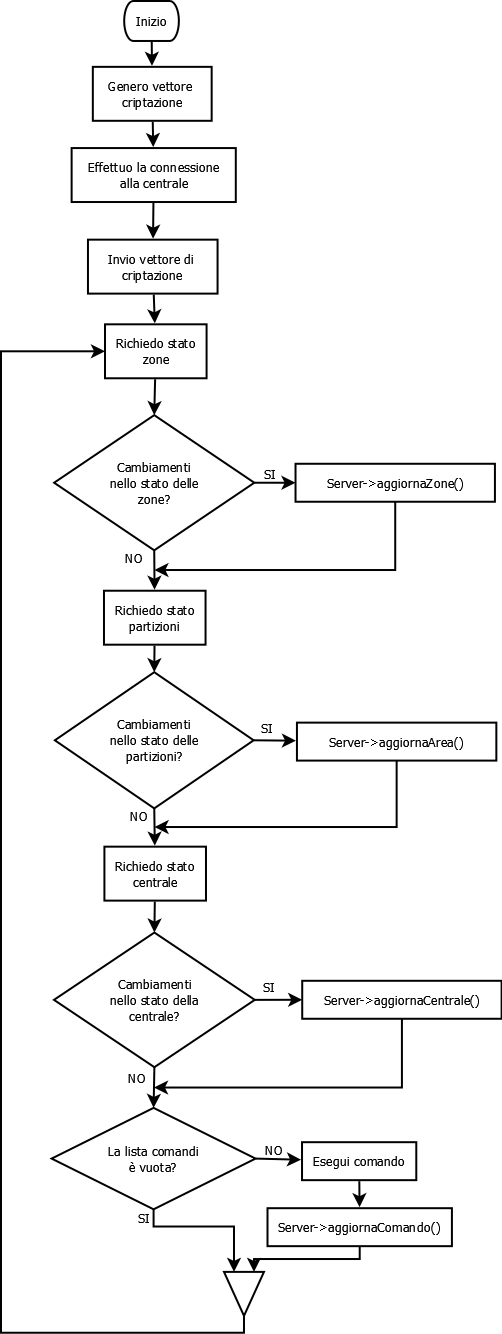
\includegraphics[width=0.7\linewidth]{pictures/runtecno.png}
	\caption{Diagramma di flusso del metodo Run della classe Tecnoalarm}\label{fig:flussotecno}
\end{figure}
\begin{lstlisting}[language=C++,caption=Costruttore della classe Tecnoalarm,label=lst:costtecno]
TecnoAlarm (long codice, Server* server);
\end{lstlisting}
Gli altri metodi della classe non fanno altro che preparare i pacchetti da trasmettere. In particolare i metodi \texttt{criptaPaccetto} e \texttt{decriptaPacchetto} sfruttano la libreria \emph{openssl}\cite{openssl} per effettuare le operazioni di criptazione e decriptazione del pacchetto. Questi due metodi sono mostrati in \lname{lst:decripta} e \lname{lst:cripta}.
\begin{lstlisting}[language=C++,caption=Metodo decriptaPacchetto,label=lst:decripta]
int TecnoAlarm::decriptaPacchetto(unsigned char * pacchetto, int len) {
    unsigned char temp[512];
    memset(temp,0,512);
    AES_cfb128_encrypt(pacchetto,temp, len, &ekey, ivtemprx, &numdec, AES_DECRYPT);
    memcpy(pacchetto,temp,len);
    return 0; 
}
\end{lstlisting}
\begin{lstlisting}[language=C++,caption=Metodo criptaPacchetto,label=lst:cripta]
int TecnoAlarm::criptaPacchetto(unsigned char * pacchetto, int len) {
    AES_cfb128_encrypt(pacchetto,pacchetto, len, &ekey, ivtemptx, &numenc, AES_ENCRYPT);
    return 0;
}
\end{lstlisting}
\subsubsection{Urmet}
Questa classe come detto eredita dalla classe \texttt{Centrale}. Il metodo \texttt{Run} si occupa solo di inviare la richiesta degli stati ed interpretare la risposta, una volta interpretata la confronta con gli stati precedenti e in caso di variazioni lo notifica al livello superiore. In \fname{fig:flussourmet} è mostrata la sequenza delle operazioni svolte dal metodo \texttt{Run}.
\begin{figure}
	\centering
	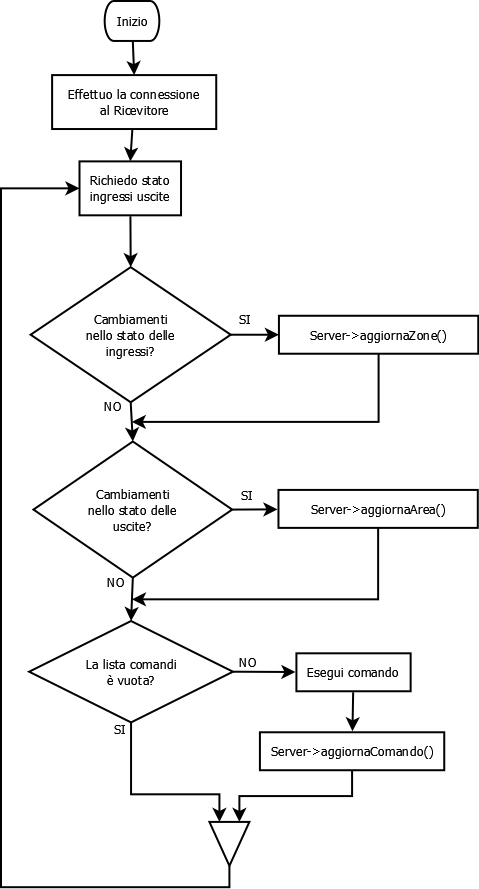
\includegraphics[width=0.7\linewidth]{pictures/teleurmet.png}
	\caption{Diagramma di flusso del metodo Run della classe Urmet}\label{fig:flussourmet}
\end{figure}
\subsubsection{Comandi}
Questa è la classica classe entità infatti essa rappresenta il generico comando, contiene due attributi che identificano il tipo di comando e l'elemento sul quale applicarlo.
\begin{lstlisting}[language=C++,caption=Classe Comandi, label=lst:comandi]
#ifndef COMANDI_H
#define COMANDI_H
enum enum_Comandi {
    ARM_PARTITION,
    DISARM_PARTITION,
    ARM_PARTIAL_PARTITION,
    INCLUDE_ZONE,
    EXCLUDE_ZONE,
    BLOCK_PROGRAM,
    UNBLOCK_PROGRAM };
class Comandi {
    public:
        Comandi (enum_Comandi comando, int elemento);
        virtual ~Comandi ();
        enum_Comandi getComando();
        int getElemento();
    private:
        enum_Comandi tipo_comando;
        int num_elemento;
};
\end{lstlisting}
%\chapter{Telegestione E-Pro}
\label{capitolo6}
\thispagestyle{empty}
In questo capitolo analizzeremo quella parte di software, trascurata nel capitolo precedente, che riguarda la comunicazione tra il software di telegestione e il server JBoss. In particolare questo tipo di comunicazione non riguarda altro che l'implementazione di un protocollo di comunicazione tra i due moduli.
\section{Il protocollo di comunicazione}
Questo tipo di protocollo in realtà non è altro che lo scambio di stringhe di messaggi tra i moduli JBoss e il software \texttt{Telegestore}, e quindi la struttura è molto semplice; argomento più complesso invece è la comunicazione tra i due software che avviene tramite due canali diversi di comunicazione. Questa decisione è stata presa in quanto le  risposte da parte di una centrale telegestita risultano essere più lente rispetto al normale utilizzo di un qualsiasi software, utilizzando due canali di comunicazione è possibile disaccoppiare la comunicazione ed evitare il blocco del software. Sul primo canale si inviano i comandi al software di telegestione il quale risponderà immediatamente tramite un meccanismo di \emph{request-replay} in modo da restituire un feedback immediato all'operatore. Sul secondo canale, invece, si sfrutta un meccanismo di \emph{publish-subscribe} dove il \texttt{Telegestore} è colui che pubblica i contenuti mentre il JBoss è in ascolto, su questo canale vengono trasmesse tutte le informazioni riguardanti la centrale telegestita come lo stato di partizioni, di zone o l'avvenuta esecuzione di un comando. Il grafico di \fname{fig:teleJboss} mostra la comunicazione tra i software.
\begin{figure}
	\centering
	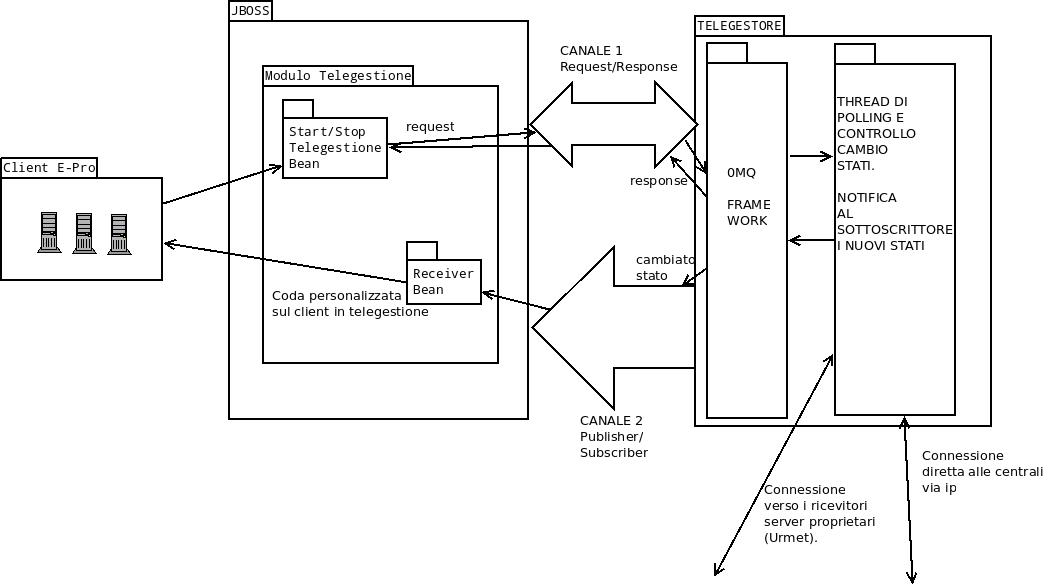
\includegraphics[width=\linewidth]{pictures/telejboss.jpeg}
	\caption{Schema di comunicazione della telegestione}\label{fig:teleJboss}
\end{figure}
\subsection{Il primo canale di comunicazione}
Il primo canale di comunicazione serve per svolgere tre compiti il primo è attivare la telegestione, il secondo disattivarla ed il terzo inviare i comandi da eseguire.
\subsubsection{La struttura del pacchetto}
La struttura del pacchetto è relativamente semplice, essa è composta da una serie di campi separati dal carattere '';'', il pacchetto è così formato:
\begin{center}
	$$ce\_id;COD;dati$$
\end{center}
\begin{description}
	\item[ce\_id:] questo campo contiene il codice identificativo della centrale;
	\item[COD:] questo campo è un codice che identifica il tipo di pacchetto e di conseguenza l'operazione da eseguire sulla centrale specificata;
	\item[dati:] questo campo ha una lunghezza variabile da 0 a 3 campi
\end{description}
Questi sono i pacchetti che il modulo eseguito sul server JBoss invia al software Telegestore, quest'ultimo risponde inviando lo stesso pacchetto ma con nel campo dati il valore \emph{OK} in caso di successo e \emph{KO} in caso di fallimento.
\subsubsection{I tipi di pacchetto}
I pacchetti che il modulo eseguito sul JBoss può inviare sono di tre tipi, il pacchetto per cominciare la telegestione, il pacchetto per interromperla e il pacchetto per eseguire il comando.\\
Il primo pacchetto di avvio della telegestione è così formattato:
$$ce\_id;AVVIO$$
quando il server lato Telegestore riceve questo comando crea un istanza di \texttt{Centrale} e ne invoca il metodo \texttt{Start} in caso tutto vada a buon fine il Telegestore risponde con il pacchetto:
$$ce\_id;AVVIO;OK$$
in caso di problemi nell'avvio della telegestione il server risponde con il messaggio:
$$ce\_id;AVVIO;KO$$
Il pacchetto di fine telegestione è simile al precedente cambia unicamente il codice comando ed il campo dati è vuoto, il pacchetto generale è:
$$ce\_id;FINE$$
Il server che riceve il messaggio invoca il metodo \texttt{Stop} sulla centrale telegestita e risponde con il messaggio:
$$ce\_id;FINE;OK$$
Il pacchetto per l'invio dei comandi contiene invece un campo dati con lunghezza diverso da 0 e il messaggio inviato è così composto:
$$ce\_id;COM;tipo;numero;comando$$
in questo caso il campo \texttt{tipo} indica il tipo di elemento sul quale applicare il comando, esso si distingue in partizione oppure zona; il campo \texttt{numero} indica il numero dell'elemento sul quale il comando deve essere eseguito, ed infine il campo \texttt{comando} indica il tipo di azione da intraprendere in base al tipo, il valore \emph{1} indica l'inserimento di una partizione oppure l'inclusione di una zona; il valore \emph{2} indica invece il disinserimento della partizione o l'esclusione della zona.\\
Il software di telegestione risponde a questo comando inserenderlo nella lista dei comandi da eseguire ed inviando il messaggio:
$$ce\_id;COM;OK$$
\subsubsection{La connessione}
La connessione avviene tramite l'utilizzo del framework ZeroMQ\cite{zmq} il quale in questo caso implementa un meccanismo di request-replay ovvero il client, il modulo JBoss, invia al server, il software Telegestore, un messaggio; il framework si preoccupa di far in modo che il messaggio arrivi a destinazione correttamente ed effettua eventuali conversioni nel tipo di dato. In questo tipo di paradigma il client non può inviare altri messaggi fino a quando il server non risponde allla prima richiesta. Questo meccanismo permette una sincronia di comunicazione tra i due software e ci permette di rispondere sempre all'ultima richiesta effettuata. In \fname{fig:contteljboss} vediamo come i due software si scambiano i messaggi.
\begin{figure}
	\centering
	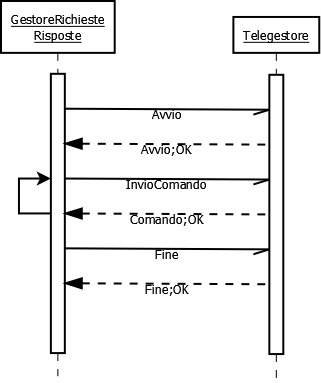
\includegraphics[width=0.5\linewidth]{pictures/congesttele.png}
	\caption{Scambio di messaggi sul canale request-replay}\label{fig:contteljboss}
\end{figure}
Un particolare di questo tipo di meccanismo è che il client risulta bloccato fino a quando non riceve una risposta e questo, in caso di invio di un comando richiederebbe diverso tempo se dovessimo aspettare l'esecuzione di tale comando sulla centrale. Per questo motivo si è deciso di inviare la conferma del comando non appena esso è stato preso in carico dal softwaare di telegestione e di utilizzare un secondo canale di comunicazione per segnalare l'avvenuta esecuzione del comando sulla centrale.
\subsection{Il secondo canale di comunicazione}
Il secondo canale di comunicazione è utilizzato per inviare al modulo in esecuzione sul JBoss gli esiti dei comandi ed eventuali variazioni degli stati degli elementi sulle centrali. Questo tipo di comunicazione avviene tramite un meccanismo di \emph{publish-subscribe} dove il Telegestore è colui che pubblica mentre il modulo JBoss si occupa di ricevere gli eventi delle centrali telegestite.
\subsubsection{La struttura del pacchetto}
I pacchetti utilizzati per lo scambio di informazioni sul secondo canale di comunicazione sono di due tipi, il primo serve per scambiare informazioni riguardo lo stato degli elementi della centrale di allarme ed è composto dai seguenti elementi:
$$ce\_id;tipo;numero;n1;n2;n3$$
nei quali gli elementi sono tutti valori numerici, in particolare il \texttt{ce\_id} serve ad individuare la centrale da cui arriva l'informazione, \texttt{tipo} è un valore numerico che serve ad indicare se si tratta di informazioni riguardanti la centrale, una partizione o una zona, il \texttt{numero} identifica il numero dell'elemento ed infine i valori \texttt{n1}, \texttt{n2} e \texttt{n3} sono dei numeri che indicano lo stato degli elementi. Il secondo tipo di pacchetto è quello che serve ad inviare le informazioni riguardo la corretta esecuzione di un comando, in questo caso la struttura del pacchetto è la seguente:
$$ce\_id;tipo;elemento;numero;comando;OK$$
oppure
$$ce\_id;tipo;elemento;numero;comando;KO$$
dove \texttt{ce\_id} è l'identificativo della centrale, \texttt{tipo} è fisso al valore 3 per indicare un pacchetto di comando, \texttt{elemento} indica il tipo di elemento sul quale il comando è stato eseguito, \texttt{numero} è il numero dell'elemento sul quale il comando viene eseguito  e \texttt{comando} è un valore che indica la tipologia di comando eseguita ed infine il la stringa \emph{OK} o \emph{KO} indicano rispettivamente se il comando è stato o non è stato eseguito.
\subsubsection{I tipi di pacchetto}
Analizziamo ora i tre tipi di pacchetto per lo scambio di informazioni riguardanti gli stati e il pacchetto per l'invio dell'esito dei comandi
\paragraph{Lo stato della centrale}
Il pacchetto che ci permette di analizzare lo stato della centrale ha la struttura:
$$ce\_id;tipo;numero;n1;n2;n3$$
Il valore del campo \texttt{tipo} è \emph{0} ed il valore del campo \texttt{numero} è solitamente \emph{1} anche se in rari casi possono esserci diverse centrali collegate tra loro. I campi \texttt{n1}, \texttt{n2} e \texttt{n3} indicano rispettivamente lo stato dell'alimentazione, della batteria e del tamper, essi possono assumere i valori \emph{-1} che indica che l'elemento non ha uno stato definito, \emph{0} che l'elemento è in uno stato di riposo ed infine \emph{1} che indica che il corrispettivo elemento è in allarme.
\paragraph{Lo stato della partizione}
Per indicare lo stato di una partizione si utilizza lo stesso pacchetto utilizzato per comunicare lo stato della centrale tuttavia il campo \texttt{tipo} questa volta assume il valore \emph{1} e i tre campi \texttt{n1}, \texttt{n2} e \texttt{n3} indicano rispettivamente se la partizione è in allarme se è inserita e se è inserita parzialmente sempre utilizzando i tre valori \emph{-1, 0} e \emph{1}.
\paragraph{Stato della zona}
Per inviare informazioni riguardo allo stato della zona si utilizza il pacchetto precedentemente mostrato con il valore \emph{2} nel campo \texttt{tipo} esso indica che le informazioni seguenti riguardano la zona numerato con il valore contenuto in \texttt{numero} le informazioni che vengono comunicate dai campi \texttt{n1}, \texttt{n2} e \texttt{n3} sono rispettivamente se la zona è in allarme, se è esclusa o se è manomessa.
\paragraph{Pacchetto di comando}
Il pacchetto di comando come abbiamo visto in precedenza è diverso da quelli di comunicazione degli stati, esso è formato come segue:
$$ce\_id;tipo;elemento;numero;comando;OK$$
dove \texttt{tipo} è sempre uguale al valore \emph{3}, \texttt{elemento} è un numero che indica se il comando è eseguito su di una zona, su di una partizione oppure su di un programmatore orario, \texttt{numero} indica il numero dell'elemento sul quale il comando è stato eseguito ed infine \texttt{comando} indica il tipo di operazione eseguita.
\subsubsection{La connessione}
Per quanto riguarda la connessione avviene tramite l'utilizzo del framework ZeroMQ\cite{zmq} che crea una connessione di tipo \emph{publish-subscribe}, in particolare la pubblicazione di un nuovo messaggio viene eseguita dalle singole istanze di \texttt{Centrale} del software di \texttt{Telegestore} che ad ogni cambiamento di stato di una zona, di una partizione o della centrale inviano tramite questa connessione un messaggio verso i moduli del JBoss.
Questo meccanismo permette di avere una connessione completamente asincrona e permette al resto del software di  procedere con la normale esecuzione.
\section{La struttura dati}
Per poter tener traccia delle operazioni eseguite e dei comandi andati a buon fine si è deciso di memorizzare sul database i comandi ed il loro stato in modo tale che in caso di crash del sistema sia possibile risalire agli eventi andati a buon fine e di quelli rimasti in sospeso.\\
Questo meccanismo non è indispensabile per il corretto funzionamento del sistema tuttavia è utile per risalire alle operazioni eseguite e per tenere traccia di eventuali problemi.
La tabella realizzata a tale scopo è quella in \lname{lst:tabcodici2}
\begin{lstlisting}[language=SQL,caption=Tabella comandi,label=lst:tabcodici2]
CREATE TABLE comandi
(
cd_id integer NOT NULL DEFAULT nextval(('"comandi_cd_id_seq"'::text)::regclass),
cd_tipo_comand integer,
cd_tipo_element integer,
cd_num_element integer,
cd_stato character(1) DEFAULT 'n'::character varying,
cd_risposta integer DEFAULT 0,
cd_centrale character varying(5),
cd_codice_hw character varying(30),
CONSTRAINT cd_comandi_id_pkey PRIMARY KEY (cd_id)
)
\end{lstlisting}
dove i campi sono autoesplicativi, il campo stato indica se il comando è stato preso in gestione dal Telegestore mentre il campo risposta indica la risposta che esso comunica al modulo JBoss. I campi \texttt{cd\_element} e \texttt{cd\_command} sono rispettivamente i campi associati ai valori che vengono trasmessi dai pacchetti inviati sul secondo canale di trasmissione.
\section{Architettura e realizzazione del sistema}
In questa sezione tratteremo la progetazione e la realizzazione della comunicazione tra il software Telegestore e i moduli in esecuzione sul JBoss; in particolare, a differenza dei capitoli precedenti non analizzeremo l'intero software ma solamente alcune classi. Per il software \texttt{Telegestore} analizzeremo la classe \texttt{Server} già mostrata nello schema delle classi di \fname{fig:classitele} mentre per quanto riguarda il modulo in esecuzione sul server JBoss analizzeremo la parte di codice che gestisce il canale \emph{request-replay} e quella che gestisce il canale \emph{public-subscribe}.
\subsection{Le classi}
In questo caso analizzeremo solo le singole classi e non l'intera struttura del software, in particolare per il software \texttt{Telegestore} analizzeremo la classe \texttt{Server}, mentre per il modulo in esecuzione sul JBoss analizzeremo le classi \texttt{GestioneRichiesteRisposte} e \texttt{ReceiverThread} che si occupano rispettivamente del primo e del secondo canale di comunicazione
\subsubsection{Server}
Questa classe, la cui struttura è mostrata in \fname{fig:serverclass} fa parte del software \texttt{Telegestore}. Questa classe si occupa di gestire interamente la connessione con il modulo JBoss che gestisce della telegestione, oltre a questo essa si occupa di creare le istanze della classe \texttt{Centrale} e di mettere in esecuzione il metodo \texttt{Run} di quest'ultima.
\begin{figure}
	\centering
	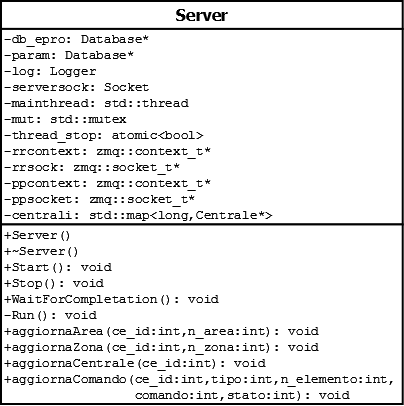
\includegraphics[width=0.5\linewidth]{pictures/serverclass.png}
	\caption{Schema della classe \texttt{Server}}\label{fig:serverclass}
\end{figure}
Il metodo \texttt{Run} della classe \texttt{Server} si occupa di gestire la comunicazione sul primo canale, esso rimane in attesa di un messaggio di richiesta, se questo messaggio è un messaggio di avvio della telegestione questo metodo crea e mette in esecuzione un'istanza di \texttt{Centrale} in base al tipo di centrale da telegestire, nel caso in cui il messaggio arrivato sia un comando il metodo \texttt{Run} ricerca la centrale all'interno della sua lista e aggiunge il comando alla sua coda di comandi; nel caso in cui il messaggio pervenuto sia di tipo “fine telegestione” questo metodo invoca il metodo \texttt{Stop} della classe \texttt{Centrale}, ne richiama il distruttore e la elimina dalla lista delle centrali. Dopo ogni operazione invia una risposta al modulo che ha inviato la richiesta.\\
Oltre ai consueti metodi di servizio già visti in tutte le classi, ovveto \texttt{Start}, \texttt{Stop} e \texttt{WaitingForCompletation} che servono a gestire il thread troviamo i metodi:
\begin{itemize}
	\item \texttt{aggiornaArea}
	\item \texttt{aggiornaZona}
	\item \texttt{aggiornaCentrale}
	\item \texttt{aggiornaComando}
\end{itemize}
Che servono per la comunicazione sul secondo canale, infatti questi quattro metodi non fanno altro che prelevare le informazioni passate come parametri interpretarle e creare il pacchetto corrispondente ed inviarlo pubblicarlo sul secondo canale di comunicazione al JBoss.
\subsubsection{GestioneRichiesteRisposte}
\begin{figure}
	\centering
	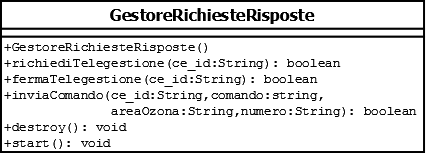
\includegraphics[width=0.5\linewidth]{pictures/classgestore.png}
	\caption{Classe \texttt{GestoreRichiesteRisposte}}\label{fig:gestricclass}
\end{figure}
Questa classe si occupa della gestione della comunicazione di tipo \emph{request-replay}, i suoi metodi vengono invocati da un livello più alto del software che noi non tratteremo.\\
Lo schema della classe è mostrato in \fname{fig:gestricclass} nel quale sono mostrati i metodi principali e non l'intera struttura della classe, tali metodi sono abbastanza facili da comprendere; il metodo \texttt{richiediTelegestione} riceve in ingresso il codice identificativo della centrale da telegestire, esso crea la connessione sul canale \emph{request-replay}, invia il comando di inizio telegestione ed attende la risposta positiva del server. Il metodo \texttt{fermaTelegestione} riceve come parametro il codice identificativo della centrale e con tale codice crea il pacchetto per fermare la telegestione, lo invia sul primo canale di comunicazione ed attende la risposta la quale sarà comunicata al livello superiore del software tramite il valore restituito dal metodo.\\
Il metodo \texttt{inviaComando} riceve come parametri di ingresso il codice identificativo della centrale, il comando da eseguire, il tipo di elemento sul quale eseguirlo e il numero dell'elemento. In particolare esso riceve i parametri direttamente nello standard del protocollo e non è quindi necessario tradurre tali dati per creare il messaggio da inviare; dopo aver preparato il pacchetto lo invia sul canale e si mette in attesa della risposta.
\subsubsection{ReceiverThread}
Questa classe si occupa della ricezione dei messaggi sul canale di trasmissione \emph{publish-subscribe}. Essa implementa un thread messo in esecuzione quando esiste almeno una sessione attiva di telegestione e si preoccupa solamente di ricevere i messaggi, non di decifrarli, essi vengono immessi in una coda la quale verrà svuotata ad un livello superiore del software nel quale verranno anche decifrati.\\
Questa classe estende la classe \texttt{Thread} e quindi non necessità dell'implementazione di altri metodi oltre al metodo \texttt{run}.
\subsection{Implementazione}
Per quanto riguarda il la classe \texttt{Server} essa è stata implementata in C++ come il resto del software Telegestore utilizzando lo standard del 2011 (ISO/IEC 14882:2011\cite{c++11}) in modo da supportare il multi-threading  in modo nativo, per fare ciò si è deciso di utilizzare il compilatore gcc-4.8, la più completa al momento in cui abbiamo sviluppato.\\
Per quanto riguarda le due classi in esecuzione sul server JBoss sono state sviluppate utilizzando il linguaggio Java aggiornato alla versione 1.5; questa scelta è stata obbligata dal resto del software in esecuzione che sfrutta dei metodi deprecati e un comportamento scorretto della stessa implementazione di Java e che quindi non può essere aggiornato. Inoltre lo stesso JBoss\cite{jboss} utilizzato non permette un aggiornamento all'ultima versione del linguaggio Java in quanto la versione utilizzata dell'application server è la 4.\\
Per quanto riguarda la camunicazione tra la classe \texttt{Server} e le due classi in esecuzione sul server JBoss è stato utilizzato il framework \emph{ZeroMQ}\cite{zmq} aggiornato alla versione 1.3 questo framework permette la creazione di diversi patern di comunicazione come il \emph{request-replay} utilizzato per il primo canale o il \emph{public-subscribe} utilizzato per il secondo senza doverci preoccupare di gestire la connessione o di controllare il corretto invio e ricezione dei messaggi.
\subsubsection{Server}
Questa classe si divide in due parti, la prima parte composta dal metodo \texttt{Run} e dai metodi che gestiscono il thread si occupa dello scambio dei messaggi sul primo canale di comunicazione, quello di tipo request-replay. Il funzionamento del metodo \texttt{Run} è molto semplice come si nota dal diagramma in \fname{fig:flussoserver}, il metodo si pone in attesa di un messaggio, in caso sia un messaggio di inizio esso invoca la creazione di una nuova istanza della classe \texttt{Centrale} e su questa istanza invoca il metodo \texttt{Start} nel caso in cui invece sia un messaggio di fine telegestione allora il metodo controlla la lista delle centrali ed elimina la centrale richiesta. Nel caso in cui, infine, il messaggio arrivato sia un messaggio di richiesta comando, allora il metodo crea un nuovo \texttt{Comando} e lo inserisce nella lista dei comandi adeguata.
\begin{figure}
\centering
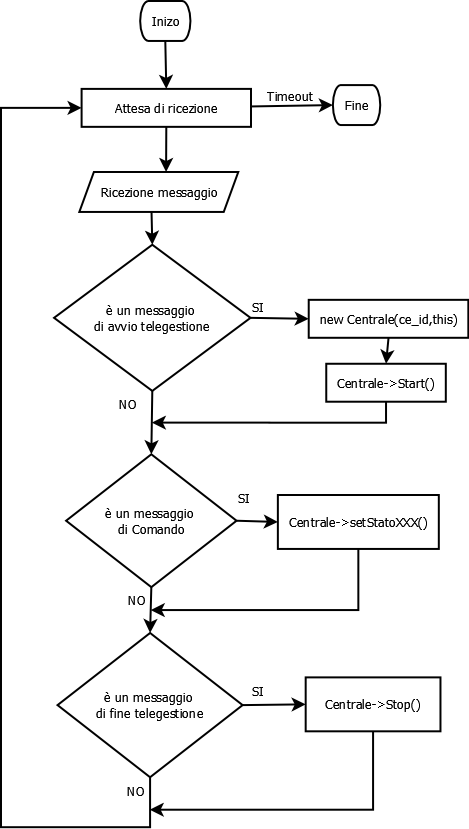
\includegraphics[width=0.7\linewidth]{pictures/flussoserver.png}
\caption{Diagramma di flusso per il metodo \texttt{Run} della classe \texttt{Server}}\label{fig:flussoserver}
\end{figure}
Per quanto riguarda la seconda parte della classe essa si occupa della trasmissione dei messaggi sul secondo canale di trasmissione ed è composta dai quattro metodi:
\begin{itemize}
	\item \texttt{aggiornaArea}
	\item \texttt{aggiornaZona}
	\item \texttt{aggiornaCentrale}
	\item \texttt{aggiornaComando}
\end{itemize}
essi hanno un comportamento molto simile tra loro e non fanno altro che utilizzare i dati passati come parametro e costrutire il pacchetto che sarà successivamente inviato sul canale publish-subscribe, come possiamo vedere dal codice mostrato in \lname{lst:aggiornacode}.
\begin{lstlisting}[language=C++,caption=Metodo aggiornaXXX,label=lst:aggiornacode]
void Server::aggiornaZona(int ce_id, int n_zona) {
    std::string risposta;
    std::map<long, Centrale *>::iterator it;
    unsigned char stato;
    it = centrali.find(ce_id);
    if(it != centrali.end()) {
        stato = it->second->getStatoZone(n_zona);
        if (stato == 0xFF) {
            risposta=std::to_string(ce_id)+";1;"+std::to_string(n_zona)+";-1;-1;-1";
        } else {
            risposta=std::to_string(ce_id)+";1;"+std::to_string(n_zona)+";"+std::to_string(stato&0x01)+";"+std::to_string(stato&0x02)+";"+std::to_string(stato&0x04);
        }
    } else {
        risposta=std::to_string(ce_id)+";1;"+std::to_string(n_zona)+";-1;-1;-1";
    }
    cout<<"Risposta: "<<risposta<<endl;
    s_sendmore(*ppsock, "005");
    s_send(*ppsock, risposta);
}
\end{lstlisting}
\subsubsection{GestoreRichiesteRisposte}
Questa classe si occupa dell'invio dei messaggi sul canale \emph{request-replay} e viene invocata da un livello superiore del software in esecuzione sul server JBoss. Essa è composta da tre metodi principali:
\begin{itemize}
	\item \texttt{richiediTelegestione}
	\item \texttt{fermaTelegestione}
	\item \texttt{inviaComando}
\end{itemize}
Questi metodi sono molto simili ed hanno lo stesso comportamento, ovvero alla loro invocazione essi stabiliscono la connessione ed invano il messaggio, dopodiché si mettono in attesa di una risposta, un esempio è il codice del metodo \texttt{fermaTelegestione} mostrato nel \lname{lst:fermatele}
\lstinputlisting[language=JAVA,caption=Metodo fermaTelegestione,label=lst:fermatele]{listati/fineTelegestione.java}
L'unica differenza si presenta nel metodo \texttt{inviaComando} il quale ha diversi parametri in ingresso tutti utilizzati per creare il pacchetto da inviare ma il comportamento del metodo rimane invariato.
\subsubsection{ReceiverThread}
Questa classe estende l'oggetto Java \texttt{Thread} per questo essa implementa il metodo \texttt{run}, in questo caso è l'unico metodo implementato oltre al costruttore. In particolare esso si occupa di ricevere il messaggio dal canale \texttt{publish-subscribe} di convertirlo in una stringa e di inserirlo in una coda che poi sarà svuotata ed analizzata ad un livello superiore del software. Il codice del metodo \texttt{run} è mostrato in \lname{lst:runpublish}.
\begin{lstlisting}[language=JAVA,caption=Metodo run,label=lst:runpublish]
public void run() {
    subscriber.connect("tcp://192.168.5.188:5556");
    String subscription = "005";
    subscriber.subscribe(subscription.getBytes());
    try {
        while (!this.isInterrupted()) {
            System.out.println("In attesa di messaggi");
            String topic = subscriber.recvStr();
            if (topic == null)
                break;
            String data = subscriber.recvStr();
            System.out.println("RICEVUTO MESSAGGIO " + data);
            TextMessage message = null;
            try {
                message = queueSession.createTextMessage();
                message.setText(data);
                queueSender.send(message);
            } catch (JMSException e) {
                e.printStackTrace();
            }
        }
    } catch (ZMQException e) {
        e.printStackTrace();
    }
}
\end{lstlisting}
%\chapter{Testing e valutazione dei risultati}
\label{capitolo7}
\thispagestyle{empty}
In questo capitolo vedremo le diverse fasi di testing e analizzeremo gli effetti del nuovo software sulle tempistiche di integrazione e in termini di aumento del numero di collegamenti effettuati con la centrale operativa.
\section{Testing}
La fase di testing del software si può dividere in tre sotto-fasi che analizzeremo in maniera distinta tuttavia facciamo una breve premessa riguardo all'architettura utilizzata per il testing.
\subsection{L'architettura del testing}
Per testare il nuovo software sono state create una serie di macchine virtuali per replicare esattamente l'architettura di produzione; inoltre, per quanto riguarda i ricevitori, la modularità del nuovo software ha permesso di escludere i ricevitori non necessari o quelli ampiamente testati. Per testare la ricezione degli allarmi si avevano a disposizione fisicamente le centrali di allarme a banco.\\
Ogni software è stato pensato per essere analizzato a diverso livello, infatti, ogni software sfrutta il demone \emph{syslog} dell'ambiente linux per scrivere diversi file di log, inoltre lo stesso demone permette di impostare il livello di log in base a sette livelli i quali servono a distinguere i messaggi più gravi da quelli necessari solo all'analisi del software. Inoltre tutto il software è stato pensato per un ulteriore divisione dei messaggi, infatti è possibile impostare il software in modo da decidere se è necessario scrivere sul file di log anche le query eseguite sul database o effettuare il log di un singolo ricevitore o telegestore.
\subsection{La prima fase di testing}
In una prima fase di testing il nuovo software viene testato singolarmente in modo da escludere l'interazione con il resto del sistema. Il nuovo software viene introdotto nell'ambiente di test, e gli unici processi eseguiti sono quello del database sul quale il nuovo software si appoggia ed il software stesso. Prendendo in considerazione, ad esempio, il software di ricezione degli allarmi e volendo testare un nuovo ricevitore, si disabilitano tutti gli altri ricevitori in modo che gli unici thread in esecuzione siano quello del controllore e quello del nuovo ricevitore da testare. A questo punto tramite una centrale d'allarme a banco si effettuano dei test controllati, in primo luogo si verifica lo stato della connessione e la corretta comunicazione dei messaggi tramite il file di log del ricevitore. Nel caso in cui la comunicazione non avvenisse in modo corretto si utilizzano diversi strumenti per l'analisi dei messaggi tra i quali \emph{Wireshark}\cite{wireshark}.\\
In caso di successo, invece, si passava a testare la validità del software ovvero, ad analizzare se gli eventi ricevuti vengono convertiti in un allarme vero e proprio dal software; per fare ciò si testano un sottoinsieme di eventi normalmente generati da una centrale d'allarme, in particolare si testano:
\begin{itemize}
	\item inserimento e disinserimento di una partizione;
	\item esclusione od inclusione di una zona;
	\item manomissione della centrale;
	\item manomissione di un sensore.
	\item Allarme di una zona
\end{itemize}
In particolare per le ultime due tipologie di segnalazioni ci serviamo di un hardware che sfrutta la configurazione dei sensori a \emph{doppio bilanciamento} in particolare in \fname{fig:sensdoppio} vediamo lo schema elettrico del collegamento di un sensore collegato in doppio bilanciamento, mentre in \fname{fig:schemadoppio} vediamo lo schema del nostro hardware, intervenendo sul contatto di \emph{tamper} si testa la manomissione del sensore mentre intervenendo sul \emph{contatto d'allarme} si testa l'allarme della zona.
\begin{figure}
	\centering
	\subfigure[]{
		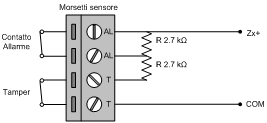
\includegraphics[width=0.4\linewidth]{pictures/doppiobilanciamento.png}\label{fig:sensdoppio}
	}
	\subfigure[]{
		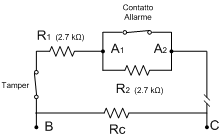
\includegraphics[width=0.4\linewidth]{pictures/b24-schema2.png}\label{fig:schemadoppio}
	}
	\caption{Configurazione di un sensore in doppio bilanciamento e schema dell'hardware di test}
\end{figure}
Per quanto riguarda il software di telegestione la fase di testing procede nello stesso modo fino a questo punto, ovvero verifica della connessione e del corretto scambio di informazioni; la validazione tuttavia consiste nel verificare il corretto invio dei comandi alla centrale e in secondo luogo la corretta traduzione degli elementi della centrale. In particolare i comandi che vengono controllati sono:
\begin{itemize}
	\item inserimento e disinserimento di una partizione;
	\item inclusione o esclusione di una zona;
\end{itemize}
Gli stati monitorati sono:
\begin{itemize}
	\item per la centrale: lo stato dell'alimentazione elettrica, lo stato della batteria e lo stato del contatto di manomissione;
	\item per le partizioni: lo stato di inserimento o di disinserimento o di inserimento parziale;
	\item per le zone: lo stato di allarme, lo stato di riposo o lo stato di esclusione
\end{itemize}
Una volta verificato il corretto funzionamento del software si passa a testare l'affidabilità mantenendo in esecuzione il software per almeno una giornata e generando periodicamente un evento o inviando un comando.\\
Nel caso in cui anche questa fase di test sia superata si testa il sistema nel suo insieme attivando anche il resto dei moduli non necessari anche nell'ambiente di test. Se anche in questo caso non si verificano errori il sistema è ritenuto abbastanza stabile e affidabile da poter essere rilasciato in produzione.
\subsection{$\alpha$-testing}
Dopo che il software ha superato la prima fase di testing si passa alla seconda nella quale la nuova versione del programma viene rilasciata sulle macchine di produzione. Dopo aver caricato l'eseguibile si programmano gli script di controllo per monitorare e, in caso di malfunzionamento, riavviare il software. In caso di crash inoltre questi sistemi di controllo inviano una mail per tenere traccia del momento esatto del riavvio. Tramite questo meccanismo è possibile risalire nel file di log all'evento che ha scatenato il blocco del sistema senza mantenere monitorato il file.\\
In questa fase il nuovo software viene avviato nell'architettura di produzione e lasciato in esecuzione, ad esso vengono collegate diverse centrali le quali tuttavia sono sempre centrali di prova collegate all'interno dell'azienda per poter intervenire in modo rapido e completo sulla centrale e cercare un riscontro dell'evento che ha eventualmente generato il crash del sistema. In questo modo è possibile testare il sistema con un carico di eventi sempre basso ma che comunque impegna il sistema anche in modo concorrente permettendo così di individuare eventuali problemi di concorrenza tra i thread.
Per quanto riguarda il \texttt{Telegestore}, invece, permette di studiare il comportamento con sensori situati in un ambiente reale anche se controllato.\\
Essendo questo test effettuato in ambiente di produzione gli eventi ricevuti dalle centrali collegate a questo ricevitore verrebbero mostrati agli operatori, per evitare ciò è possibile selezionare un parametro nella configurazione della centrale nel software E-Pro che permette di registrare gli allarmi sul database ma di renderli passanti ovvero di non mostrarli agli operatori.\\
Lo scopo principale di questo tipo di testing è quello di individuare problemi di concorrenza e di verificare in modo più approfondito la stabilità del sistema il quale è un requisito fondamentale per questi software.
\subsection{$\beta$-testing}
Alla fine della fase di $ \alpha$-test il nuovo software è già in produzione e risulta abbastanza stabile, tuttavia il numero di segnalazioni o di gestioni è molto ridotto in quanto il numero di centrali collegate è inferiore a dieci mentre a pieno ritmo i collegamenti possibili sono anche dell'ordine delle migliaia di centrali.\\
Per progredire nel testing del software si passa alla fase di $ \beta$-test nella quale vengono collegate al nuovo ricevitore diverse centrali selezionate tra quelle già installate dai clienti in modo da avere un numero più elevato di segnalazioni anche contemporanee provenienti almeno da un centinaio di centrali.\\
Questa fase è un vero e proprio stress test del nuovo software il quale deve essere in grado di sopportare il carico delle segnalazioni o delle telegestioni.\\
In questo caso le segnalazioni vengo gestite dagli operatori e siamo quasi nella situazione di normale funzionamento, tuttavia rispetto alla situazione standard le centrali selezionate come $ \beta$-tester dispongono anche di un sistema di backup che è in grado di inviare le segnalazioni di allarme anche tramite un altro vettore e quindi destinate ad un ricevitore diverso da quello testato.\\
Durante questa fase si individuano eventuali problemi di concorrenza su larga scala, eventuale sottodimensionamento delle risorse del ricevitore ed eventuali errori di traduzione degli allarmi.
\section{Valutazione dei risultati}
Analizziamo ora in termini numerici quali sono stati i miglioramenti che il nostro lavoro ha portato all'interno dell'azienda. In particolare possiamo analizzare i miglioramenti in termini di velocità di integrazione e\emph{ “time to market”}, analizzando la riduzione delle tempistiche di gestione delle segnalazioni ed il carico del sistema, infine possiamo fare riferimento anche all'aumento del numero di collegamenti alla centrale.\\
In particolare per quanto riguarda la fase di integrazione possiamo distinguere due tempistiche, la prima che ha riguardato la fase di progettazione del software che ha richiesto all'incirca quattro mesi ma che si è svolta un'unica volta e la seconda tempistica che si ha ogni qualvolta che si deve integrare un nuovo protocollo di ricezione che è nell'ordine di due settimane dal momento della ricezione del protocollo al termine della prima fase di testing, in base alla complessità del protocollo. Prima del nostro intervento questa fase poteva richiedere anche alcuni mesi a causa della complessità della logica del software precedentemente creato che non permetteva l'inserimento di un nuovo ricevitore senza interferire con il resto del codice.\\
Per quanto riguarda la riduzione dei tempi di gestione è dovuta a due fattori principali, la riduzione dei tempi di trasmissione degli eventi e la riduzione dei tempi di gestione degli operatori tramite l'utilizzo della telegestione. Per quanto riguarda la riduzione dei tempi di trasmissione si è passati da un tempo di trasmissione dell'ordine dei \emph{20s} in caso di comunicazione su PSTN ad un tempo inferiore ai \emph{2s} per trasmissioni tramite TCP/IP inoltre, il ricevitore PSTN poteva ricevere fino a dieci comunicazioni simultanee, con un ricevitore software il numero di connessioni simultanee è stato limitato a 250 per singolo ricevitore. Per quanto riguarda invece, la vera e propria gestione dell'evento da parte degli operatori, si è notato un riduzione del 20\% dei tempi di gestione soprattutto grazie alla telegestione che permette di eseguire le operazioni più comuni sulle centrali direttamente dal software E-Pro senza dover cambiare postazione per accedere al software di telegestione specifico per il tipo di centrale.\\
Una diretta conseguenza della facilità di integrazione di nuovi ricevitori e della telegestione di nuove centrali è l'aumento del numero di collegamenti con la centrale operativa e il conseguente aumento del numero di clienti; questo aumento è quantificabile con il 10\% in più dei clienti gestiti.

\cleardoublepage
% ---- Bibliography ----
\addcontentsline{toc}{chapter}{Bibliografia}
\printbibliography
%\nocite{*}

\appendix

\pagestyle{fancy} 
\fancyfoot{}                                               
\renewcommand{\chaptermark}[1]{\markboth{\appendixname\ \thechapter.\ #1}{}} 
\renewcommand{\sectionmark}[1]{\markright{\thesection.\ #1}}         
\fancyhead[LE,RO]{\bfseries\thepage}    
                                        
\fancyhead[RE]{\bfseries\leftmark}    
\fancyhead[LO]{\bfseries\rightmark}     
\renewcommand{\headrulewidth}{0.3pt} 

\chapter{Documentazione del progetto logico}
\label{appendiceA}
\thispagestyle{empty}

\noindent Documentazione del progetto logico dove si documenta il progetto logico del sistema e se \`e il caso si mostra la progettazione in grande del SW e dell'HW. Quest'appendice mostra l'architettura logica implementativa (nella Sezione 4 c'era la descrizione, qui ci vanno gli schemi a blocchi e i diagrammi).
%\include{appendiceB}
%\include{appendiceC}
%\include{appendiceD}
%\include{appendiceE}
%\include{appendiceF}

\end{document}





